\documentclass[12pt, twoside, a4paper]{report}
\usepackage[bindingoffset=2cm,centering,includeheadfoot,margin=2.8cm]{geometry}
\usepackage[cm-default]{fontspec}
\setromanfont{FreeSerif}
\usepackage{xunicode}
\usepackage{indentfirst}
\usepackage{xltxtra}
\usepackage{xgreek}
\usepackage{listings}
\usepackage[usenames, dvipsnames]{color}
%%\usepackage{caption}
\usepackage{cite}
%%\usepackage{float}
%%\usepackage{amsmath}
%%\usepackage{graphicx}
%%\usepackage{algorithmicx}
%%\usepackage{array}
%%\usepackage{tabularx}
%%\usepackage{subcaption}
%%\usepackage{comment}
\usepackage{hyphenat}

\setmainfont[Mapping=tex-text]{DejaVu Serif}
\setmonofont[Mapping=tex-text]{DejaVu Sans Mono}

%%\captionsetup[lstlisting]{labelfont=bf,textfont=normalfont}
%%\captionsetup[figure]{labelfont=bf,textfont=normalfont}
%%\captionsetup[table]{labelfont=bf,textfont=normalfont}
%%\lstset{basicstyle=\footnotesize\ttfamily}

\setcounter{secnumdepth}{5}
%%\pagestyle{headings}
%%\usepackage[dvips]{graphicx}
\usepackage{hyperref}
%%\hypersetup{
%%    colorlinks=true, %set true if you want colored links
%%    linkcolor=black,  %choose some color if you want links to stand out
%%}

\begin{document}

\lstset{
	language=C,                % choose the language of the code
	numbers=left,                   % where to put the line-numbers
	stepnumber=1,                   % the step between two line-numbers.        
	numbersep=5pt,                  % how far the line-numbers are from the code
	backgroundcolor=\color{white},  % choose the background color. You must add \usepackage{color}
	basicstyle=\ttfamily,
	keywordstyle=\color{Maroon}\ttfamily,
	stringstyle=\color{blue}\ttfamily,
	commentstyle=\color{Gray}\ttfamily,
	morecomment=[l][\color{ForestGreen}]{\#}
	showspaces=false,               % show spaces adding particular underscores
	showstringspaces=false,         % underline spaces within strings
	showtabs=false,                 % show tabs within strings adding particular underscores
	tabsize=8,                      % sets default tabsize to 2 spaces
	captionpos=b,                   % sets the caption-position to bottom
	breaklines=true,                % sets automatic line breaking
	breakatwhitespace=true,         % sets if automatic breaks should only happen at whitespace
	title=\lstname,                 % show the filename of files included with \lstinputlisting;
}
\renewcommand*{\lstlistingname}{Code}

%%\title{
\addtolength{\topmargin}{-0.5in}
\thispagestyle{empty}
\vspace{-8ex}
\begin{center}

\includegraphics[scale=1]{figures/pyrforos.eps}
\end{center}
\begin{center}
\Large{Ε}\large{ΘΝΙΚO}
\Large{Μ}\large{ΕΤΣOΒΙΟ}
\Large{Π}\large{ΟΛΥΤΕΧΝΕIΟ} \\
\normalsize{Τ}\small{ΜΉΜΑ}
\normalsize{H}\small{ΛΕΚΤΡΟΛΟΓΩΝ}
\normalsize{M}\small{ΗΧΑΝΙΚΩΝ}
\normalsize{K}\small{AI}
\normalsize{M}\small{ΗΧΑΝΙΚΩΝ}
\normalsize{Y}\small{ΠΟΛΟΓΙΣΤΩΝ} \\
\vspace{2ex}
-ΕΙΣΑΓΕΤΕ ΤΟΝ ΤΟΜΕΑ- \\
-ΕΙΣΑΓΕΤΕ ΤΟ ΕΡΓΑΣΤΗΡΙΟ- \\
\end{center}
\begin{center}
\vspace{8ex}
\large \textbf{-Εισάγετε τον τίτλο της διπλωματικής εργασίας-} \\
\vspace{10ex}
\large
ΔΙΠΛΩΜΑΤΙΚΗ ΕΡΓΑΣΙΑ\\
\vspace{2ex}
\normalsize
-Εισάγετε το σωστό άρθρο (της/του/των)- \\
\end{center}
\vspace{2ex}
\begin{center}
\parbox[c]{0.4\textwidth} { \center\textbf{
-Εισάγετε το όνομα, αρχικό πατρώνυμου και επώνυμο των συγγραφέων- }}
\parbox[c]{0.4\textwidth} { \center\textbf{
	-another author, whose name is here- }}
\vspace{10ex}
\end{center}
%%\flushleft
\begin{tabbing}
	\textbf{Επιβλέπων}: \= -Εισάγετε το όνομα, αρχικό πατρώνυμου
				και επίθετο- \\
			    \> -Εισάγετε τον τίτλο του επιβλέποντα-
\end{tabbing}
%%}
%%\date{
\begin{center}
\normalsize
Αθήνα, -Εισάγετε το μήνα και το έτος κατάθεσης της εργασίας-
%%}
\end{center}

%%\maketitle
\newpage
\thispagestyle{empty}
\hspace{10pt}
%\tiny
%(this page is left intentionally blanc)
%\normalsize
\newpage
\thispagestyle{empty}

\includegraphics[scale=1.1]{figures/pyrforos.eps}
\noindent
\parbox[b]{0.7\textwidth} {\textbf{
\noindent
\normalsize{ΕΘΝΙΚΌ}
\normalsize{ΜΕΤΣΌΒΙΟ}
\normalsize{ΠΟΛΥΤΕΧΝΕΊΟ}} \\
\small
TMHMA
ΗΛΕΚΤΡΟΛΟΓΩΝ
ΜΗΧΑΝΙΚΩΝ
ΚΑΙ
ΜΗΧΑΝΙΚΩΝ
ΥΠΟΛΟΓΙΣΤΩΝ \\
-ΕΙΣΑΓΕΤΕ ΤΟΝ ΤΟΜΕΑ- \\
-ΕΙΣΑΓΕΤΕ ΤΟ ΕΡΓΑΣΤΗΡΙΟ- \\
}

\begin{center}
\vspace{7ex}
\large \textbf{-Εισάγετε τον τίτλο της διπλωματικής εργασίας-} \\
\vspace{8ex}
\large
ΔΙΠΛΩΜΑΤΙΚΗ ΕΡΓΑΣΙΑ\\
\vspace{2ex}
\normalsize
-Εισάγετε το σωστό άρθρο (της/του/των)- \\
\vspace{2ex}
\parbox[c]{0.4\textwidth} { \center\textbf{
-Εισάγετε το όνομα, αρχικό πατρώνυμου και επώνυμο των συγγραφέων- }}
%%\parbox[c]{0.4\textwidth} { \center\textbf{
%%	-another author, whose name is here- }}
\vspace{10ex}
%%\flushleft
\begin{tabbing}
	\textbf{Επιβλέπων}: \= -Εισάγετε το όνομα, αρχικό πατρώνυμου
				και επίθετο- \\
			    \> -Εισάγετε τον τίτλο του επιβλέποντα-
\end{tabbing}
\end{center}

\noindent
Εγκρίθηκε από την τριμελή εξεταστική επιτροπή την -εισάγετε ημερομηνία-.

\begin{center}
\scriptsize
\parbox[b]{0.3\textwidth} {\center
	........................................
	-Εισάγετε ονοματεπώνυμο-
	-Εισάγετε τίτλο-
}
\parbox[b]{0.3\textwidth} {\center
	........................................
	-Εισάγετε ονοματεπώνυμο-
	-Εισάγετε τίτλο-
}
\parbox[b]{0.3\textwidth} {\center
	........................................
	-Εισάγετε ονοματεπώνυμο-
	-Εισάγετε τίτλο-
}
\end{center}
\vspace{10ex}
\normalsize
\noindent
Αθήνα, (Εισάγετε το μήνα και το έτος κατάθεσης της εργασίας).
\newpage
\thispagestyle{empty}
\hspace{10pt}

\vspace{30ex}
\noindent
................................... \\
\textbf{(Εισάγετε όνομα, αρχικό πατρώνυμου και επίθετο συγγραφέα)} \\
(Εισάγετε τον απονεμηθέντα τίτλο του συγγραφέα) \\
\vspace{8ex}

%%\noindent
%%................................... \\
%%\textbf{(Εισάγετε όνομα, αρχικό πατρώνυμου και επίθετο συγγραφέα)} \\
%%(Εισάγετε τον απονεμηθέντα τίτλο του συγγραφέα) \\
%%\vspace{8ex}
%%
%%\noindent
%%................................... \\
%%\textbf{(Εισάγετε όνομα, αρχικό πατρώνυμου και επίθετο συγγραφέα)} \\
%%(Εισάγετε τον απονεμηθέντα τίτλο του συγγραφέα) \\
%%\vspace{26ex}

\small
\noindent
\copyright \hspace{1em}(Εισάγετε έτος έκδοσης) Εθνικό Μετσόβιο Πολυτεχνείο.
All rights reserved.

\renewcommand{\abstractname}{Περίληψη}

\begin{abstract}
Τα τελευταία χρόνια το cloud computing αποτελεί ένα σημαντικό κεφάλαιο στη
σύγχρονη επιστήμη υπολογιστών. Η κύρια τεχνολογία που χρησιμοποιείται,
	προκειμένου να μπορεί να υποστηριχθεί το cloud computing είναι αυτή της
	εικονικοποίησης. Με αυτό τον τρόπο ένα φυσικό μηχάνημα, μπορεί να
	φιλοξενήσει πολλά εικονικά μηχανήματα, κάθε ένα από τα οποία αποτελεί
	έναν αυτοδύναμο υπολογιστή. Ωστόσο, αποτελεί συχνό φαινόμενο οι
	εικονικές αυτές μηχανές να χρησιμοποιούνται για την εκτέλεση μίας και
	μόνο εφαρμογής. Αυτό έχει ως αποτέλεσμα, να χαραμείζονται πόροι σε
	ενέργειες που δε χρειάζονται από την εφαρμογή, αλλά είναι απαραίτητες
	για το λειτουργικό σύστημα στο οποίο τρέχουν αυτές οι εφαρμογές. 
	
Μία νεότερη τάση για την υποστήριξη του cloud computing είναι τα
	containers, που προσφέρουν ελαφρύτερη εικονικοποίηση με γρηγορους
	χρόνους εκτέλεσης, μικρή κατανάλωση μνήμης και άλλα πλεονεκτήματα. Από
	την άλλη, παρουσιάζουν αρκετά σημαντικά ζητήματα που
	αφορούν την ασφάλεια. Ένα από τα ζητήματα αυτά είναι, εκείνο της
	απομόνωσης το οποίο αναγκάζει σε αρκετές περιπτώσεις να οδηγεί στη χρήση
	εικονικών μηχανών για τη φιλοξενία των containers, χάνοντας αρκετά από
	τα πλεονεκτήματα τους.  

Μία ακόμη προσέγγιση στο θέμα είναι οι unikernels. Πρόκειται για μία εικόνα
	εικονικής μηχανής, με ένα μόνο address space το οποίο κατασκευάζεται από
	library operating systems και είναι ειδικευμένο για μία συγκεκριμένη
	εφαρμογή. Πιο απλά, περιέχει τον κώδικα της εφαρμογής και ακριβώς ό,τι
	κομμάτι του λειτουργικού συστήματος χρειάζεται η εφαρμογή για να
	λειτουργήσει η διεργασία (drivers, βιβλιοθήκες, κ.λ.π.), ενοποιημένα 
	σαν ένα	αυτόνομο πρόγραμμα που μπορεί να τρέξει ως εικονική μηχανή.
	Οι unikernels καταφέρνουν να έχουν γρήγορους χρόνους εκκίνησης και μικρή
	κατανάλωση μνήμης, χωρίς να θυσιάζεται η ασφάλεια
	Εν τούτοις, ένα πρόβλημα είναι ότι οι unikernels υποστηρίζουν μία και
	μόνο διεργασία, με αποτέλεσμα να μην μπορούν εφαρμογές με παραπάνω από
	μία διεργασίες να εκτελεστούν σε unikernels. 

Σκοπός, λοιπόν, αυτής της εργασίας είναι η υλοποίηση ενός μηχανισμού που θα
	επιτρέπει σε εφαρμογές με περισσότερες από μία διεργασίες να μπορούν να
	εκτελεστούν και σε unikernels. Επιπλέον, υλοποιείται και ένας απλός
	μηχανισμός για επικοινωνία μεταξύ των εικονικών μηχανών, στα πρότυπα του pipe. 
\vspace{2ex}

Λέξεις-Κλειδιά: εικονικοποίηση, εικονικές μηχανές, ενδοεπικοινωνία εικονικών μηχανών, unikernel, kvm, QEMU
\end{abstract}

\renewcommand{\abstractname}{Abstract}

\begin{abstract}
In recent years cloud computing is one important chapter of modern commputer
	science. The main technology used in order to support cloud computing is
	virtualization. Virtualization makes possible for a physical machine to
	host many virtual machines, each one of which is a self-sufficient
	computer. However, virtual machines are often used to execute a single
	application. As a result, resources are devoted to actions that are not
	needed by the application, but they are necessary for the operating
	system in which the applications run.

An another technology to support cloud computing is containers which offer
	lightweight virtualization, fast instantiation times and small
	per-instance 
	memory footprints among other features. On the other hand, containers
	have several important security issues. Isolation is one of these issues
	, which in several cases leads to the use of virtual machines to host
	the containers, losing several of their advantages.

A further approach in cloud computing is unikernerls. Unikernels are
	specialised, single-address-space machine images constructed by using
	library operating systems and are specialised for one application. In
	somewhat simplified terms, unikernels consist of the application's
	source code and the parts of an opperating system that are necessary for
	the proccess to run (drivers, libraries, etc.) consolidated as a
	stand-alone virtual machine. The Unikernels manage to have fast
	instantiation times, small memory footprints, without sacrificing
	security. However, one of the problems of unikernels is that they are
	single-proccess and as a result multi-proccess applcations are not able
	to run on unikernels. 

The purpose of this thesis is to implement a mechanism that will enable the
	execution of multi-proccess applications on unikernels. Furthermore, a
	pipe-like mechanism for inter-vm communication is impemented.
\vspace{2ex}

Keywords: virtualization, virtual machines, inter-vm communication, unikernel, kvm, QEMU
\end{abstract}



\newpage
\thispagestyle{empty}
\mbox{}
\newpage

\setcounter{page}{1}
\tableofcontents
\newpage
\listoffigures
%%\numberwithin{lstlisting}{chapter}
%%\numberwithin{figure}{chapter}

\chapter{Εισαγωγή}
Στις μέρες μας το cloud computing έχει γίνει ένα από τα ταχύτερα αναπτυσσόμενα
και ενδιαφέροντα θέματα στην επιστήμη των υπολογιστών. Το cloud computing δίνει
τη δυνατότητα σε απομακρυσμένους χρήστες να αποκτάνε πρόσβαση σε υπολογιστικούς
πόρους (αποθηκευτικός χώρος, εφαρμογές, υπηρεσίες κ.λ.π.) όταν χρειαστούν από
τους χρήστες. Ιδιαίτερα, τα τελευταία χρόνια το cloud έχει μπει και στις ζωές
των απλών χρηστών. H χρήση των προσωπικών υπολογιστών αρχίζει να αλλάζει
σημαντικά, καθώς πλέον προγράμματα και δεδομένα απομακρύνονται από τους 
προσωπικούς υπολογιστές για να εκτελεστούν και να αποθηκευτούν στο λεγόμενο
cloud. 

Μία από τις βασικές τεχνολογίες που κρύβονται πίσω από το cloud είναι αυτή της
εικονικοποίησης. Χάρις την εικονικοποίηση, μπορούμε σε ένα φυσικό μηχάνημα να
φιλοξενήσουμε πολλά εικονικά μηχανήματα κάθε ένα από τα οποία είναι ανεξάρτητο.
Με αυτό τον τρόπο, μπορούμε να αξιοποιήσουμε καλύτερα τους φυσικούς πόρους του
μηχανήματος και να τους διαμοιράσουμε όπως επιθυμούμε μεταξύ των εικονικών
μηχανών. Ακόμα, η εικονικοποίηση δημιούργησε και κάποιες νέες δυνατότητες, όπως
αυτή της μεταφοράς εικονικών μηχανών σε διαφορετικό φυσικό μηχάνημα, η
δημιουργία αντιγράφων εικονικών μηχανών, αλλά και περισσότερη ασφάλεια, αφού ένα
πρόβλημα σε ένα εικονικό μηχάνημα δε θα επηρεάσει ούτε το φυσικό ούτε τα
υπόλοιπα εικονικά μηχανήματα. 

Ένα συχνό φαινόμενο κατά τη χρήση της εικονικοποίησης, είναι η χρήση μία
εικονικής μηχανής με συμβατικά λειτουργικά συστήματα για την υποστήριξη μίας και
μόνο υπηρεσίας. Όπως είναι φυσικό το λειτουργικό σύσστημα μέσα στην εικονική
μηχανή χρειάζεται κάποιους πόρους για να λειτουργήσει, ενώ συχνά μπορεί να
εκτελεί λειτουργίες οι οποίες δε χρειάζονται από την εφαρμογή. Ακόμα, ο κώδικας
όλου του λειτουργικού συστήματος αυξάνει αρκετά και το μέγεθος σε μνήμη της
εικονικής μηχανής. Γϊνεται λοιπόν, κατανοητό ότι σπαταλούνται πόροι, οι οποίοι
θα μπορούσα να διατεθούν είτε στην ίδια την υπηρεσία είτε σε κάποια άλλη. 

Για την επίλυση του παραπάνω προβλήμαατος αναζητήθηκαν λύσεις για να γίνει η
εικονικοποίηση πιο ελαφρυά, αλλά και να μη σπαταλούνται πόροι σε αχρείαστες
λειτουργίες. Μία από αυτές τις λύσεις, ήταν η εικονικοποίηση σε επίπεδο
λειτουργικού συστήματος ή διαφορετικά containerization. Με τη συγκεκριμένη
μέθοδο ο πυρήνας επιτρέπει την ύπαρξη πολλαπλών απομονωμένων user-space
instances, που ονομάζονται containers. Τα containers μοιράζονται μεταξύ τους το
λειτουργικό σύστημα στα οποία εκτελούνται, ενώ ταυτόχρονα παρέχουν ένα
απομονωμένο περιβάλλον για τις διεργασίες μέσα σε αυτό. 

Η τεχνολογιά των containers, όπως κάθε άλλη τεχνολογιά δε θα μπορούσε να μην
έχει και κάποια μειονεκτήματα. Ένα από τα κύρια μειονεκτήματα, είναι αυτό της
ασφάλειας. Τα containers μοιράζοντααι τον ίδιο πυρήνα του host, ενώ οι
μηχανισμοί απομόνωσης δεν είναι το ίδιο ισχυροί με αυτούς στα εικονικά
μηχανήματα. Μάλιστα, έχουν αναφερθεί περιπτώσεις όπου από ένα container
μπορούσαν να παρθούν πληροφορίες και δεδομένα τόσο για το host, όσο και για άλλα
containers ~\cite{gao2017containerleaks}. Όλα αυτά έχουν οδηγήσει σε περιπτώσεις
όπου τα containers χρησιμοποιούνται πάνω από ένα πλήρη λειτουργικό σύστημα το
οποίο τρέχει μέσα σε μία εικονική μηχανή.

Μία ιδέα που αρχίζει να αποκτά όλο και περισσότερο ενδιαφέρον και προσοχή 
είναι αυτή των unikernels. Η βάση της ιδέας, είναι  η
κατασκευή ειδικευμένω εικονικών μηχανών για κάθε ξεχωριστή υπηρεσία. Στην
εικονική αυτή μηχανή δε χρειάζεται να υπάρχει ένα πλήρη λειτουργικό σύστημα,
αλλά μόνο τα κομμάτια αυτού τα οποία είναι απαραίτητα για την εκτέλεση της
υπηρεσίας. Με αυτό τον τρόπο, μειώνεται σημαντικά το μέγεθος των εικονικών
μηχανών, ενώ πλέον οι πόροι χρησιμοποιούνται ακριβώς για τις λειτουργίες που
χρειάζεται η υπηρεσία. Τέλος, εφόσον αναφερόμαστε σε εικονικές μηχανές, η
απομόνωση τους είναι κάτι το οποίο έχουν φροντίσει ήδη οι ελεγκτές. 

\section{Σκοπός}

Η φιλοσοφία των unikernels είναι ότι κάθε εικονική μηχανή θα έχει ένα
συγκεκριμένο σκοπό. Για το λόγο αυτό οι unikernels δεν υποστηρίζουν παραπάνω
από μία διεργασία σε κάθε εικονική μηχανή. Από την άλλη, υπάρχουν unikernel
frameworks τα οποία επιτρέπουν την υποστήριξη περισσότερων από ένα νήμα. Ωστόσο
οι περισσότερες εφαρμογές και υπηρεσίες στο cloud είναι φτιαγμένες για ένα πλήρη
λειτουργικό σύστημα. Επομένως, προκειμένου να μπορούν να τρέξουν σε ένα
unikernel θα πρέπει να αλλάξει άλλοτε περισσότερο και άλλοτε λιγότερο ο
σχεδιασμός τους. Ιδιαίτερα, οι εφαρμογές που χρησιμοποιούν παραπάνω από μία
διεργασίες θα πρέπει να αλλάξουν σε ένα μοντέλο με μία μόνο διεργασία. 

%%Η φιλοσοφία των unikernels είναι ότι κάθε εικονική μηχανή θα έχει ένα
%%συγκεκριμένο σκοπό, συνεπώς δε χρειάζονται παραπάνω από μία διεργασίες, ενώ δεν
%%υπάρχει διαχωρισμός ανάμεσα σε kernelspace και userspace. Άλλωστε πρόκειται για
%%ειδικευμένες εικονικές μηχανές που θα υποστηρίζουν ακριβώς μία υπηρεσία,
%%κάνοντας έτσι τους μηχανισμούς αυτούς του λειτουργικού συστήματος περιττούς.
%%Ωστόσο, το μεγαλύτερο μέρος των εφαρμογών και υπηρεσιών, έχουν φτιαχτεί με σκοπό
%%να τρέχουν σε πλήρη λειτουργικά συστήματα, χρησιμοποιώντας νήματα και διεργασίες
%%για την εκτέλεση τους. Ενώ υπάρχουν unikernels frameworks που υποστηρίζουν
%%περισσότερα από ένα thread, εφαρμογές που χρησιμοποιούν παραπάνω από μία
%%διεργασία, χρειάζονται να αλλάξουν για να μπορέσουν να τρέξουν σε κάποιο
%%unikernel framework. 

Ο σκοπός της συγκεκριμένης εργασίας είναι να υλοποιήσει, κρατώντας τo
single-proccess χαρακτηριστικό των unikernels, ένα μηχανισμό για την υποστήριξη
των εφαρμογών που απαιτούν παραπάνω από μία διεργασία. 

Αρχικά έγινε μία μελέτη γύρω από τα υπάρχοντα unikernel frameworks, παρατηρώντας
τα χαρακτηριστικά του κάθε ενός. Στη συνέχεια σε ένα από αυτά τα unikernels
(rumprun) υλοποιήθηκαν οι δύο παρακάτω λειτουργίες:

\begin{itemize}
\item ένας μηχανισμός για επικοινωνία μεταξύ των vms, ο οποίος είναι στα πρότυπα
της κλήσης συστήματος pipe (POSIX). Ουσιαστικά πρόκειται για την υλοποίηση της
pipe σε επίπεδο εικονικών μηχανών. 
\item  ένας μηχανισμός για την υποστήριξη της κλήσης συστήματος fork από τους
unikernels. Όταν μία εφαρμογή θα χρησιμοποιεί τη συγκεκριμένη κλήση συστήματος,
θα δημιουργείται μία νέα εικονική μηχανή κλώνος της αρχικής και θα ξεκινά την
εκτέλεση της, ακριβώς μετά την κλήση συστήματος fork.
\end{itemize}

\section{Οργάνωση Κειμένου}
Στη συνέχεια παρουσιάζεται αναλυτικά η περιγραφή του σχεδιασμού και της
υλοποίησης των δύο λειτουργιών pipe, fork, γίνεται μία ανασκόπηση στα ήδη
υπάρχοντα unikernel frameworks και περιγράφεται το απαραίτητο θεωρητικό υπόβαθρο.

Πιο συγκεκριμένα, στο Κεφάλαιο 2 καλύπτεται το απαραίτητο θεωρητικό υπόβαθρο,
κάνοντας μία μικρή αναφορά για το cloud computing, μία εισαγωγή στην εικονικοποίηση και στα λειτουργικά συστήματα.

Στο Κεφάλαιο 3 παρουσιάζονται τα unikernel frameworks που μελετήθηκαν, τα
χαρακτηριστικά τους, η φιλοσοφία τους κ.λ.π.

Στο Κεφάλαιο 4 γίνεται αναλυτική περιγραφή του σχεδιασμού και της υλοποίησης των
δύο λειτουργιών που αναφέρθηκαν προηγουμένως στο σκοπό της εργασίας (pipe,
fork).

Τέλος,στο Κεφάλαιο 6 αναφέρονται τα τελικά συμπεράσματα της παρούσας μελέτης
όπως επίσης και πιθανές μελλοντικές επεκτάσεις αυτής της διπλωματικής εργασίας.


\chapter{Θεωρητικό Υπόβαθρο}
\label{chap:background}

\section{Cloud computing}
Εδώ και αρκετό καιρό γίνεται συχνά ανφορά στο "Cloud", αλλά και σε αυτή την
εργασία έχει αναφερθεί αρκετές φορές ο όρος "cloud computing". Παρά τη δημοφιλία
του όρου, δεν υπάρχει ακριβής ορισμός. Εντούτοις, θα χρησιμοποιηθεί ο ορισμός
που έχει δωθεί από το NIST (National Institute of Standards and Technology of
USA) ~\cite{mell2011nist}. Το cloud computing (υπολογιστικό νέφος με ελληνικούς
όρους) είναι η κατ' αίτηση διαδικτυακή κεντρική διάθεση υπολογιστικών πόρων
(όπως δίκτυο, εξυπηρετητές, εφαρμογές και υπηρεσίες) με υψηλή ευελιξία, ελάχιστη
προσπάθεια από τον χρήστη και υψηλή αυτοματοποίηση. Ωστόσο, είναι συχνό
φαινόμενο να αναφερόμαστε με το συγκεκριμένο όρο τόσο στις υπηρεσίες που είναι
διαθέσιμες μέσω διαδικτύου με τη μορφή μίας υπηρεσίας ιστού όσο και στο υλικό
και λογισμικό που απαρτίζουν την υποδομή που προσφέρει αυτές τις υπηρεσίες. 

\subsection{Χαρακτηριστικά του cloud computing}

Πέρα από τον ορισμό το NIST~\cite{mell2011nist}, περιγράφει και τα ακόλουθα
βασικά χαρακτηριστικά του cloud computing: 

\begin{itemize}
\item παροχή υπηρεσίας κατ’ απαίτηση: Οι χρήστες έχουν τη δυνατότητα να
τροποποιήσουν τους πόρους που προσφέρονται, χωρίς την ανθρώπινη διαμεσολάβηση
από την πλευρά του παρόχου του cloud. 
\item ευρυζωνική δικτυακή πρόσβαση: Οι υπηρεσίες είναι διαθέσιμες από το
διαδίκτυο.
\item Διάθεση πόρων σε περισσότερους χρήστες: Οι πόροι μπορούν να διατεθούν
ανάμεσα σε πολλούς χρήστες χωρίς να δημιουργούνται προβλήματα.
\item ταχεία ελαστικότητα/επεκτασιμότητα: Οι πόροι μπορούν να ανακατεμηθούν,
είτε αυτόματα είτε κατ' απαίτηση, χωρίς περιορισμούς και χωρίς να επηρεάζεται η
ομαλή λειτουργία άλλων υπηρεσιών.
\item μετρήσιμη υπηρεσία: Η χρήση των πόρων καταγράφεται και παρουσιάζεται τόσο
στον πάροχο όσο και στον πελάτη.
\end{itemize}

\subsection{Μοντέλα υπηρεσιών}

Σύμφωνα με το NIST~\cite{mell2011nist}, τα μοντέλα υπηρεσιών του cloud είναι τα
εξής:

\vspace{2ex}
\underline{Λογισμικό ως Υπηρεσία (SaaS)}

\vspace{1ex}
Η υπηρεσία που παρέχεται στο χρήστη είναι αυτή μία εφαρμογής που τρέχει  στην
υποδομή του παρόχου. Ο χρήστης δε χρειάζεται να γνωρίζει τίποτα σχετικά με την
υποδομή που υποστηρίζει την εφαρμογή, ούτε έχει τη δυνατότητα να τροποποιήσει
πολλά πράγματα πέρα ίσως από κάποιες ρυθμίσεις που προσφέρει η εφαρμογή. Οι
εφαρμογές αυτές είναι προσβάσιμες μέσα από κάποιο λογιμικό πελάτη που προσφέρει
ο πάροχος ή ακόμα και από ένα πειηγητή ιστού (web browser).

\vspace{2ex}
\underline{Πλατφόρμα ως υπηρεσία (PaaS)}

\vspace{1ex}
Σε αυτή την περίπτωση ο χρήστης έχει τη δυνατότητα της δημιουργίας εφαρμογών
ή/και περιβάλλοντων εφαρμογών, χρησιμοποιώντας προγραμματιστικά εργαλεία και
υπηρεσίες που παρέχονται από τον πάροχο. Ο χρήστης δεν μπορεί να ελέγξει και να
διαχειριστεί την υποδομή του cloud, ωστόσο έχει τον έλεγχο των αναπτυγμένων
εφαρμογών και ενδεχομένως των ρυθμίσεων διαμόρφωσης για το περιβάλλον φιλοξενίας
αυτών των εφαρμογών.

\vspace{2ex}
\underline{Υποδομή ως υπηρεσία (IaaS)}

\vspace{1ex}
Οι παροχές προς το χρήστη είναι υπολογιστικοί πόροι όπως επεξεργαστές,
αποθηκευτικός χώρος και δίκτυο στα οποία μπορεί αναπτύξει και να τρέξει
λειτουργικά συστήματα και εφαρμογές. Παρά τη δυνατότητα να τροποποιήσει την
ποσότητα των πόρων, ο χρήστης δεν έχει παραπάνω έλεγχο ως προς την υποδομή του
cloud. 

\begin{figure}[htp]
\centering
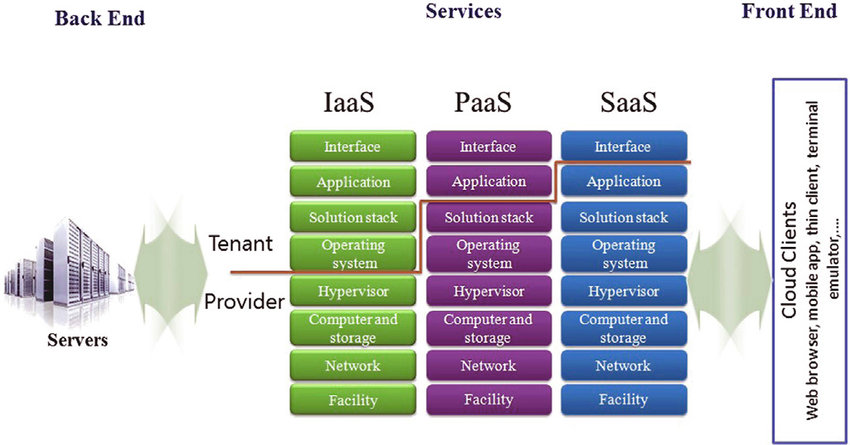
\includegraphics[scale=0.50]{figures/Cloud-service-stack.png}
\caption{Cloud services\label{fig1}}
\end{figure}

\newpage
Όπως βλέπουμε και από το σχήμα ~\ref{fig1}, όσο περισσότερη ευελιξία προσφέρει
ένα μοντέλα τόσο περισσότερο έλεγχο έχει και ο χρήστης στις υπηρεσίες που
λαμβάνει. Για παράδειγμα στην περίπτωση SaaS, ο χρήστης έχει το λιγότερο έλεγχο,
σε αντίθεση με την περίπτωση IaaS όπου ο χρήστης μπορεί πλέον να αποκτήσει
έλεγχο ακόμα και στο λειτυργικό σύστημα.

\section{Εικονικοποίηση}

Στην επιστήμη των υπολογιστών ο όρος εικονικοποίηση (\EN{virtualization}) περιγράφει
ένα μηχανισμό αφαίρεσης, που με τη χρήση "εικονικών υπολογιστικών πόρων", έχει
ως σκοπό την απόκρυψη λεπτομερειών για την υλοποίηση ή την κατάσταση των φυσικών
πόρων. Με το μηχανισμό αυτό ένας φυσικός πόρος μπορεί να παρουσιαστεί ως μία
πλειάδα εικονικών φυσικών πόρων, ή αντίστροφα μία πλειάδα φυσικών πόρων να
παρουσιαστούν ως ένας ενιαίος εικονικός πόρος. Ανάλογα σε ποιο
επίπεδο στη στοίβα του λογισμικού υλοποιείται η εικονικοποίηση, υπάρχουν και τα
αντίστοιχα πλεονεκτήματα, αλλά σε γενικές γραμμές κάποια από τα  πλεονεκτήματα
της εικονικοποίησης είναι:

\begin{itemize}
	\item Καλύτερη αξιοποίηση και διαμοιρασμός των πόρων.
	\item Ασφάλεια μεσω της απομόνωσης των υπηρεσιών.
	\item Δυνατότητα προσομοίωσης περιβαλλόντων που δεν είναι φυσικά
		διαθέσιμα.
	\item Δυνατότητα αποθήκευσης, μεταφοράς και επαναφοράς της κατάστασης
		των υπηρεσιών που προσφέρονται μέσω της εικονικοποίησης.
\end{itemize}

Η εικονικοποίηση μπορεί να υλοποιηθεί σε διάφορα επίπεδα, όπως στο δίκτυο, στον
αποθηκευτικό χώρο, στο hardware, στο λειτουργικό σύστημα κ.α. Η συγκεκριμένη
εργασία ασχολείται κυρίως με την εικονικοποίηση σε επίπεδο υλικού, ωστόσο είναι
συχό φαινόμενο να συγκρίνονται οι unikernels με τα containers. Για το λόγο αυτό
θα γίνει μία σύντομη παρουσίαση της εικονικοποίησης σε επίπεδο λειτουργικού
συστήματος, ενώ μετά από αυτή την περιγραφή, όταν χρησιμοποιείται ο όρος
εικονικοποίηση θα εννοείται εικονικοποίηση επιπέδου υλικού. 

\subsection{Εικονικοποίηση σε επίπεδο λειτουργικού συστήματος}
Η εικονικοποίηση σε επίπεδο λειτουργικού συστήματος είναι νεότερη σε σχέση με
αυτή σε επίπεδο υλικού, ωστόσο έχει καταφέρει να συγκεντρώσει αρκετή προσοχή τα
τελευταία χρόνια. Ο πυρήνας του λειτουργικού συστήματος επιτρέπει την ύπαρξη
παραπάνω από ενα, απομονωμέα userspace instances τα οποία ονομάζονται
containers, virtualization engines ή jails. Όπως φαίνεται στο σχήμα
~\ref{fig2} όλα τα containers μοιράζονται τον
ίδιο πυρήνα πάνω από τον οποίο βρίσκεται το στρώμα που είναι υπεύθυνο για την εικονικοποίηση. 

Το γεγονός ότι τα containers μοιράζονται τον ίδιο πυρήνα κάνει το μέγεθο τους
αρκετά μικρό, αφού δε χρειάζεται να συμπεριλάβουν κάποιο λειτουργικό σύστημα.
Επιπλέον, οι χρόνοι εκκίνησης τους είναι αρκετά μικροί, χωρίς να χρειάζεται να
καταναλωθεί πολύ μνήμη για τη λειτουργεία των containers. Eπιπροσθέτως, τα
containers είναι ανεξάρτητα από το φυσικό μηχάνημα, καθώς η εικονικοποίηση
γίνεται με τη χρήση του κατάλληλου λογισμικού χωρίς να χρειάζεται κάποια
υποστήριξη από το hardware. Τέλος, τα containers επιτρέπουν το εύκολο
πακετάρισμα τόσο των εφαρμογών όσο και των κατάλληλων ρυθμίσεων, που σε
συνδυασμό με την ανεξαρτησία από το hardware, δίνουν τη
δυνατότητα για την εύκολη μεταφορά τους σε διαφορετικά μηχανήματα.

\newpage
\begin{figure}[htp]
\centering
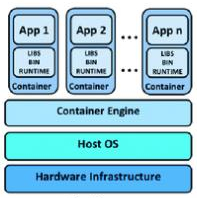
\includegraphics{figures/containers.jpg}
\caption{Εικονικοποίηση σε επίπεδο λειτουργικού συστήματος\label{fig2}}
\end{figure}

Δυστυχώς, όλα αυτά τα πλεονεκτήματα έρχονται με κάποιο κόστος, με το μεγαλύτερο
να είναι αυτό της ασφάλειας. Αν και οι υποστηρικτές των containers θεωρούν ότι
με τις κατάλληλες ρυθμίσεις τα containers μπορούν να γίνουν ασφαλή, δεν
προσφέρουν την ίδια ασφάλεια με την εικονικοποίηση σε επίπεδο
υλικού~\cite{hayden2015securing}. Τα containers δεν έχουν τη δυνατότητα να
προσφέρουν τόσο ισχυρή απομόνωση όσο προσφέρει η εικονικοποίηση σε επίπεδο
υλικού. Τα αποτελέσματα από την παραβίαση της απομόνωσης μπορεί να είναι από την
απόκτηση πληροφοριών σχετικά με το host μηχάνημα ή άλλων containers, μέχρι την
απόκτηση ελέγχου του λειτουργικού συστήματος στον
host~\cite{gao2017containerleaks}. 

Η σύγκριση τψν δύο ειδών εικονικοποίησης είναι ένα ανοιχτό ζήτημα το οποίο
δύσκολα θα λυθεί σύντομα~\cite{eder2016hypervisor}. Άλλωστε και τα δύο είδη,
αναπτύσσονται ταχύτατα, προσφέροντας συνεχώς νέες δυνατότητες και μειώνοντας τα
προβλήματα που υπάρχουν. Σε μία προσπάθεια να ενοποιηθούν τα θετικα των δύο
ειδών, είναι συχνή η χρήση εικονικών μηχανών μέσα στις οποίες τρέχουν
containers. Με αυτό τον τρόπο βελτιώνεται η ασφάλεια σε βάρος όμως της απόδοσης,
καθώς πλέον χρειάζονται πόροι και για την εκτέλεση του απαραίτητου  λογισμικού 
που θα επιτρέψει την υπάρξη εικονικών μηχανών.

\subsection{Εικονικοποίηση σε επίπεδο υλικού}

Η εικονικοποίηση σε επίπεδο υλικού, ή απλά εικονικοποίηση για το υπόλοιπο της
συγκεκριμένης εργασίας, επιτρέπει τη λειτουργία ενός ολόκληρου υπολογιστικού
συστήματος μέσα από έναν άλλον. Τα εμφωλευμένα υπολογιστικά συστήματα
αναφέρονται ως guests, ενώ το υπολογιστικό σύστημα στο οποίο πραγματοποιείται η
εικονικοποίηση αναφέρεται ως host. Ένας guest εκτελείται μέσα σε μία εικονική
μηχανή (virtual machine - VM), την οποία οι Popek και Goldberg
~\cite{popek1974formal} ορίζουν ως εξής: “ένα αποδοτικό και απομονωμένο
αντίγραφο μιας πραγματικής μηχανής”. Κάθε εικονική μηχανή είναι ανεξάρτητη τόσο
από το host, όσο και άπο άλλες τυχόν εικονικές μηχανές που μπορεί να υπάρχουν.
Με αυτού του είδους την εικονικοποίηση, κάθε εικονική μηχανή έχει την
ψαυδαίσθηση ότι κατέχει αποκλειστικά τους πόρους που της έχουν διατεθεί.

Απαραίτητο συστατικό για να επιτευχθούν όλα τα παραπάνω είναι ο επόπτης
(hypervisor). Ο επόπτης, σύμφωνα με τους Popek και Goldberg έχει τρία
συγκεκριμένα χαρακτηριστικά ~\cite{popek1974formal}:
\begin{enumerate}
	\item o επόπτης παρέχει ένα περιβάλλον όμοιο με το πραγματικό 
			υπολογιστικό σύστημα,
	\item τα προγράμματα που τρέχουν στο περιβάλλον που δημιουργείται θα
		πρέπει να έχουν στη χειρότερη περίπτωση μικρές μειώσεις στην
		ταχύτητα εκτέλεσης,
	\item o επόπτης έχει πλήρη έλεγχο των πόρων.
\end{enumerate}

Ο ρόλος του επόπτη μοιάζει με το ρόλο του λειτουργικού συστήματος, 
με τις εικονικές μηχανές να έχουν το ρόλο των διεργασιών. Ο επόπτης
χρονοδρομολογεί τις εικονικές μηχανές στη CPU, μοιράζει γενικότερα τους
διαθέσιμους πόρους στα εικονικά μηχανήματα, εκτελεί εκ μέρους των εικονικών
μηχανών "προνομιούχες εντολές" και είναι αυτός που διαχειρίζεται τις εικονικές
μηχανές (δημιουργία, εκκίνηση, τερματισμός κ.λ.π).

Όπως βλέπουμε στο σχήμα ~\ref{fig3} υπάρχουν δύο διαφορετικά είδη εποπτών,
ανάλογα με το που βρίσκονται στο σύστημα. 
\begin{itemize}
	\item \textbf{Type 1 - Bare metal/native} \\
		Σε αυτή την περίπτωση ο επόπτης εκτελείται πάνω από το υλικό του
		συστήματος, χωρίς να παρεμβάλλεται κάποιο λειτουργικό σύστημα.
		Είναι υπεύθυνος για τη χρονοδρομολόγηση των εικονικών μηχανών,
		τη διαχείριση της μνήμης και των πόρων καθώς και άλλων
		λειτουργιών. Χρησιμοποιεί δικούς του drivers για τη διαχείριση
		του υλικού και για την εξυπηρέτηση των I/O λειτουργιών των
		guest. 
	\item \textbf{Type 2 - Hosted} \\
		Σε αυτή την περίπτωση ο επόπτης εκτελείται πάνω από ένα
		λειτουργικό σύστημα, σαν ένα συνηθισμένο πρόγραμμα στο
		\EN{user space.} Αποτελούν ένα ενδιάμεσο στρώμα μεταξύ του host και
		του guest, δημιουργώντας το κατάλληλο περιβάλλον για τις
		εικονικές μηχανές. Δε χρειάζονται ειδικοί drivers για 
		το υλικό, καθώς αυτοί παρέχονται από το λειτουργικό σύστημα του
		host. Από την άλλη, οι I/O λειτουργίες και διάφορες άλλες
		"προνομιούχες εντολές" του guest θα πρέπει να
		περάσουν μέσα από τον hypervisor και μετά να εξυπηρετηθούν από
		τον host, δημιοργώντας επιπλέον κόστος στην εκτέλεση τους. 
\end{itemize}

\begin{figure}[htp]
\centering
	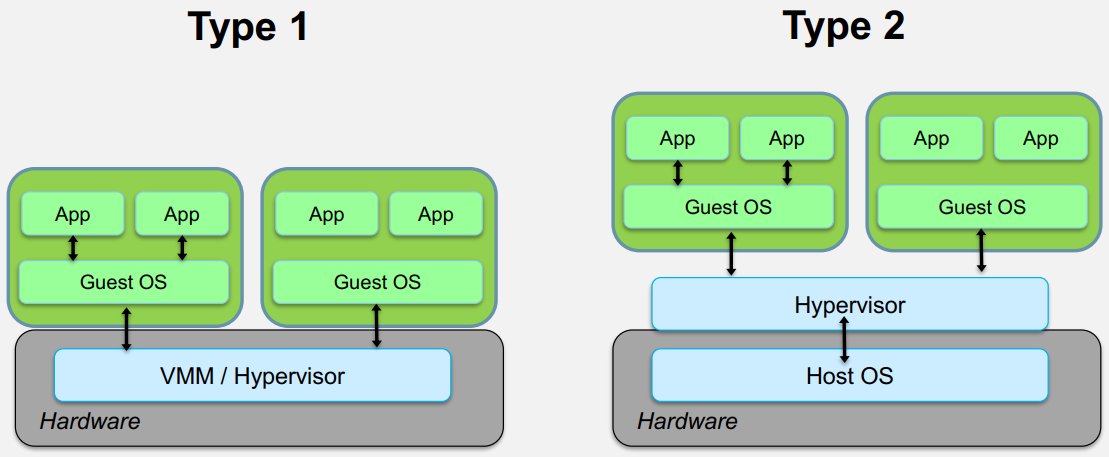
\includegraphics[scale=0.3]{figures/zcBClDR.png}
\caption{Εικονικοποίηση σε επίπεδο υλικού\label{fig3}}
\end{figure}

Εκτός από το διαχωρισμό των εποπτών, γίνεται και διαχωρισμός και στις τεχνικές
που χρησιμοποιούντα για να επιτευχθεί η εικονικοποίηση. Οι τεχνικές αυτές
βασίζονται τόσο στη δυνατότητα που προσφέρει ειδικό υλικό για την υποστήριξη της
εικονικοποίησης, όσο και στο βαθμό συνεργασίας μεταξύ του επόπτη με το εικονικό
μηχάνημα. Θα αναφερθούμε σε τρεις από αυτές τις τεχνικές, την πλήρη
εικονικοποίηση (full virtualization), την παραεικονικοποίηση
(paravirtualization) και τέλος την εικονικοποίηση υποστηριζόμενη από το υλικό
(hardware-assisted virtualization). 

\vspace{2ex}
\underline{Full virtualization}

\vspace{1ex}

Στην πλήρη εικονικοποίηση ο guest δεν έχει υποστεί καμία αλλαγή και εκτελείται
όπως και στην περίπτωση που εκτελείται απευθείας σε ένα φυσικό υπολογιστικό
σύστημα. Απο τη μεριά του ελεγκτή, θα πρέπει να γίνει πλήρης προσομοίωση του
υλικού ώστε να δίνει την ψευδαίσθηση στον guest ότι επικοινωνούν απευθείας με το
υλικό. Ωστόσο δημιουργείται ένα πρόβλημα, το λειτουργικό σύστημα του guest
εκτελείται σε unprivileged mode, οπότε δεν μπορεί να εκτελέσει προνομιούχες
εντολές. Η λύση σε αυτό το πρόβλημα είναι η τεχνική trap-and-emulate
~\cite{adams2006comparison}, κατά την οποία όταν ο guest προσπαθεί να εκτελέσει
μία προνομιούχα εντολή, δημιουργείται μία εξαίρεση (trap) στον hypervisor, καθώς
ο guest βρίσκεται σε unprivileged mode. Ύστερα, ο hypervisor παίρνει τον έλεγχο
και προσομοιώνει ή εκτελεί την προνομοιούχα εντολή για λογαριασμό του guest. 

H συγκεκριμένη λύση δεν είναι αρκετή για όλες τις αρχιτεκτονικές. Μία από αυτές
τις αρχιτεκτονικές είναι και η x86. Στην x86 αρχιτεκτονική ορισμένες εντολές
δεν προκαλούν trap όταν εκτελούνται σε unprivileged mode, παρά το γεγονός ότι
για την εκτέλεση τους είναι ανάγκη να βρίσκονται σε privileged mode
(non-virtualizable instructions). Μία από
αυτές τις εντολές είναι η popf, η οποία ενώ αλλάζει τόσο τα ALU flags όσο και τα
flags του επεξεργαστή δεν προκαλεί κάποιο trap με αποτέλεσμα να αγνοούνται οι
αλλαγές στα flags του επεξεργαστή. Για την αντιμετόπιση του συγκεκριμένου
προβλήματος χρησιμοποείται από τους επόπτες η τεχνική του binary translation
~\cite{adams2006comparison}. 
Όταν ο guest βρίσκεται σε unprivileged mode όλες οι εντολές εκτελούνται
κανονικά, ενώ όταν μεταβεί στον πυρήνα και σε privileged mode τότε ο hypervisor
μεταφράζει τις εντολές που δεν προκαλούν trap σε ένα νέο σύνολο εντολών που θα
επιφέρουν τις επιθυμητές αλλαγές στην εικονική μηχανή. 

Μπορούμε να παρατηρήσουμε εύκολα ότι και στις δύο περιπτώσεις η απόδοση θα
μειωθεί σημαντικά, λόγω της ανάμειξης του \EN{hypervisor}. Ιδιαίτερα στην περίπτωση
του binary translation το κόστος της παρακολούθησης και μετάφρασης των εντολών
του guest είναι αρκετά μεγάλο. 

\vspace{2ex}
\underline{Paravirtualization}

\vspace{1ex}

Στην παραεικονικοποίηση ο guest γνωρίζει ότι δεν εκτελείται απευθείας στο υλικό
και "συνεργάζεται" κατάλληλα με τον hypervisor. Απαιτείται λοιπόν, η τροποποίηση
του guest, ώστε να αντικατασταθούν οι non-virtualizable εντολές, με κατάλληλες
εντολές (hypercalls) που δίνουν τον έλεγχο στο hypervisor και αυτός με τη σειρά του διεκπαιρεώνει την αντίστοιχη λειτουργία. Επιπλέον ο hypervisor μπορεί να
υποστηρίξει και κάποιες άλλες εντολές, που χρησιμοποιούνται για άλλες σημαντικές
λειτουργίες του πυρήνα, όπως διαχείρηση μνήμης, διαχείριση διακοπών κ.α. 

Με αυτό τον τρόπο μειώνεται σημαντικά το κόστος της εικονικοποίησης, αφού ο
guest γνωρίζει ότι εκτελείται σε εικονικό περιβάλλον και μπορεί να
βελτιστοποιηθεί για τις συγκεκριμένες συνθήκες. Παράλληλα γίνεται
δυνατόν να εικονικοποιηθούν αρχιτεκτονικές όπως η x86 χωρίς σημαντική μείωση
της απόδοσης αποφεύγοντας το binary translation. Από την άλλη, o guest
τροποποιείται αρκετά για να μπορέσει να "συνεργαστεί" με τον επόπτη. Συνεπώς, 
μειώνεται η δυνατότητα μεταφοράς του σε διαφορετικά συστήματα (π.χ. διαφορετικό
επόπτη), ενώ ταυτόχρονα αυξάνει το κόστος συντήρησης του καθώς οποιεσδήποτε
αλλάγές ή αναβαθμίσεις στον πυρήνα του guest θα πρέπει να τροποποιηθούν
κατάλληλα για την υποστήριξη της παραεικονικοποίησης.

\vspace{2ex}
\underline{Hardware-assisted virtualization}

\vspace{1ex}

Η συγκεκριμένη μέθοδος ουσιαστικά έχει τα ίδια χαρακτηριστικά με τη μέθοδο της
πλήρης εικονικοποίησης. Ο guest δε χρειάζεται να υποστεί καμία αλλαγή, ενώ
εισάγεται κατάλληλο hardware το οποίο διευκολύνει την εικονικοποίηση. Πρόκειται
για επεκτάσεις των επεξεργαστών με στόχο την αύξηση της απόδοσης και της
ασφάλειας της εικονικοποίησης. Αυτές οι επεκτάσεις είναι γνωστές ως επεκτάσεις
εικονικοποίησης (virtualization extensions). 

Ένα από τα βασικά στοιχεία αυτών των επεκτάσεων είναι η δημιουργία ενός νέου
επιπέδου εκτέλεσης, αυτό του guest στο οποίο μπορούν να εκτελεστούν τόσο
privileged όσο και unprivileged εντολές. Συνεπώς, δε χρειάζεται πλέον να
γίνονται trap οι privileged εντολές του guest, αλλά αυτές μπορούν να εκτελεστούν
απευθείας, χωρίς μάλιστα να επηρεάζεται ο host από την εκτέλεση τους. Οι
επεκτάσεις αφορούν ακόμα τη διαχείριση μνήμης, αλλά και των διακοπών. Πλέον η
εκτέλεση του guest συνεχίζεται αδιάκοπα μέχρι την ικανοποίηση κάποιας συνθήκες,
όπως για παράδειγμα ένα page fault, όπου τότε ο έλεγχος μεταφέρεται στον host
(VM exit). 

Με αυτό τον τρόπο επιτυγχάνεται υψηλή απόδοση για την εικονικοποίηση χωρίς να
είναι απαραίτητες οι αλλαγές στον guest. O πιο σημαντικός παράγοντας απόδοσης
για την εν λόγω τεχνική είναι το πλήθος των VM exits, καθώς πρόκειται για μία
χρονοβόρα διαδικασία ~\cite{agesen2012software}. Μάλιστα πολλές από αυτές τις
επεκτάσεις έχουν δημιοργηθεί με ακριβώς αυτό το σκοπό, δηλαδή τη μείωση των VM
exits. 


\subsection{QEMU/KVM}

Το Qemu ~\cite{bellard2005qemu} είναι ένας επόπτης τύπου 2 και πρόκειται για
έναν από τους πιο γνωστούς επόπτες. Με την τεχνική του full virtualization και
συγκεκριμένα με τη μέθοδο του dynamic binary translation, υποστηρίζει τη
φιλοξενεία πολλών λειτουργικών συστημάτων χωρίς να απαιτείται κάποια αλλαγή σε
αυτά. Πέρα από τη λειτουργία του επόπτη, μπορεί να λειτουργήσει και ως
προσομοιωτής υλικού. Το Qemu έχει τη δυνατότητα να προσομοιώσει διαφορετικές
αρχιτεκτονικές από αυτή που διαθέτει ο host, πληθώρα από κάρτες δικτύου,
σκληρούς δίσκους, περιφερειακές συσκευές κ.λ.π.. Mε αυτό τον τρόπο μπορεί να
χρησιμοποιηθεί και για εφαρμογές που έχουν υλοποιηθεί για διαφορετική
αρχιτεκτονική να εκτελεστούν στην αρχιτεκτονική που διαθέτει ο host. 

Οι εικονικές μηχανές που εκτελούνται στον ίδιο host, συχνά επικοινωνούν μεταξύ
τους. Συνήθως πρόκειται για πλήρη υπολογιστικά συστήματα, συνεπώς για την
επικοινωνία μεταξύ τους θα μπορούσε να χρησιμοποιηθεί ό,τι χρησιμοποιειταί
μεταξύ φυσικών υπολογιστικών συστημάτων (π.χ. TCP/IP sockets). Μάλιστα ειδικά
στη συγκεκριμένη περίπτωση οι επόπτες μπορούν να αντιληφθούν ότι πρόκειται για
επικοινωνία μεταξύ εικονικών μηχανών που ελέγχουν οπότε και χρησιμοποιούν
διάφορες βελτιστοποιήσεις, προκειμένου να μη χρειαστεί να περάσουν τα πακέτα
πέρα από το host. Εντούτοις, συχνά πολλές εικονικές μηχανές δε χρειάζονται
δίκτυο και δημιουργείται η ανάγκη για επικοινωνία μεταξύ άλλων εικονικών μηχανών
λη ακόμα και με το host. Επιπλεόν πολλές φορές είναι χρήσιμο εικονικές μηχανές
να μοιράζονται μνήμη μεταξύ τους . Έτσι έχουν δημιουργηθεί αρκετές μέθοδοι για
τον διαμοιρασμό μνήμης και ενδοεπικοινωνίας μεταξύ εικονικών μηχανών, αλλά και
μεταξύ του host και των εικονικών μηχανών ~\cite{ren2016shared}. 

Ένας από αυτούς τους μηχανισμούς είναι ο nahanni ή ivshmem (inter-VM shared
memory) ~\cite{macdonell2011shared}. To ivshmem είναι ένας μηχανισμός για το
διαμοιρασμό μνήμης του host με τις εικονικές μηχανές που εκτελούνται στο host.
Μπορεί να χρησιμοποιηθεί τόσο για διαμοιρασμό μνήμης μεταξύ host και guest, όσο
και μεταξύ των guests. To Qemu επιτρέπει τη χρήση αυτού τού μηχανισμού μέσω
μίας PCI συσκευής την οποία πρέπει να υποστηρίξουν οι guests για να
χρησιμοποιήσουν τη συγκεκριμένη περιοχή μνήμης. 

Πολλές φορές το Qemu χρησιμοποιείται από άλλους επόπτες για την εξομοίωση του
υλικού, όπως για παράδειγμα γίνεται από το Xen. Επιπροσθέτως συχνά
χρησιμοποιείται σε συνδυασμό με το kvm (στην περίπτωση υποστήριξης
hardware-assisted virtualization), πετυχαίνοντας υψηλή απόδοση. Ωστόσο, από μόνο
του το kvm δε λειτουργεί ως επόπτης, αλλά ανοίγει μία διεπαφή (/dev/kvm) μέσω
της οποίας μπορούν να χρησιμοποιηθούν οι διάφορες λειτουργίες που προσφέρει.
Το kvm είναι ένα kernel module του Linux, που μετατρέπει τον πυρήνα σε εναν
επόπτη. Σε αυτό τον συνδυασμό (Qemu/Kvm) κάθε εικονική μηχανή εκτελείται ως μία
διεργασία. 

\section{Λειτουργικά συστήματα}

Το λειτουργικό σύστημα είναι ένα πρόγραμμα το οποίο εκτελείται σε ένα
υπολογιστικό σύστημα. Η ειδοποιός διαφορά του με οποιοδήποτε άλλο πρόγραμμα
είναι ότι το πρώτο υπάρχει για να εξυπηρετεί το δεύτερο. Το λειτουργικό σύστημα
διαχειρίζεται το υλικό του υπολογιστικού συστήματος και παρέχει στους
πργαμματιστές των εφαρμογών ένα σαφές αφηρημένο σύνολο πόρων, αντί για το
μπερδεμένο σύνολο που υπάρχει στο υπολογιστικό σύστημα. Χωρίς αυτό, ο
προγραμματιστής μίας οποιασδήποτε εφαρμογής θα έπρεπε να γράψει και τον κατάλληο
κώδικα για το υλικό που χρησιμοποιεί η συγκεκριμένη εφαρμογή (π.χ. αποθήκευση σε
σκληρό δίσκο). Ως εκ τούτου θα σπαταλούσε αρκετό χρόνο σε μη βασικές λειτουργίες
του προγράμματος. Επιπροσθέτως πολλές από αυτές τις λειτουργίες που αφορούν το
υλικό μπορεί να έχουν ήδη υλοποιηθεί από άλλα προγράμματα, σπαταλώντας έτσι
χρόνο για ήδη υπάρχουσες λειτουργίες. 

Η πληθώρα και οι σημαντικές διαφορές στο σκοπό και στις δυνατότητες των
υπολογιστικών συστημάτων οδήγησε στη δημιουργία διαφορετικών ειδών λειτουργικών
συστημάτων. Για παράδειγμα, ένα λειτουργικό σύστημα που έχει δημιουργηθεί με
σκοπό την εκτέλεση του σε προσωπικούς υπολογιστές διαφέρει αρκετά από ένα
λειτουργικό σύσστημα που χρησιμοποιείται σε ενσωματωμένα συστήματα. Το πιο
γνωστό είδος λειτουργικών συστημάτων είναι αυτά του γενικού σκοπού, τα οποία
έχουν ως στόχο να μπορούν να εκτελεστούν σε διάφορα υπολογιστικά συστήματα
προσφέροντας όσο το δυνατόν περισσότερες λειτουργίες. 

Ένας διαφορετικός τρόπος κατηγοριοποίησης των λειτουργικών συστημάτων γίνεται με
τη δομή τους. Θα αναφερθούν οι κυριότερες από αυτές τις δομές, μονολιθικά
συστήματα, πολυεπίπεδα συστήματα, μικροπυρήνες.

\begin{itemize}
	\item μονολιθικά συστήματα: η πιο διαδεδομένη οργάνωση, στην οποία
		ολόκληρουόκληρο το λειτουργικό συστημα εκτελείται ως ένα
		μοναδικό πρόγραμμα σε κατάσταση πυρήνα. Ουσιαστικά πρόκειται για
		ένα μεγάλο εκτελέσιμο δυαδικό πρόγραμμα. Κάθε διαδικασία του
		συστήματος μπορεί να καλέσει οποιαδήποτε άλλη. 
	\item πολυεπίπεδα συστήματα: το λειτουργικό σύστημα οργανώνενται σε μία
		ιεραρχία επιπέδων, όπου το καθένα δομείται πάνω στο αμέσως
		κατώτερο του. Κάθε επίπεδο αναλαμβάνει μία διαφορετική
		λειτουργία και μπορεί να χρησιμοποιείσει μόνο λειτουργίες που
		υποστηρίζουν κατώτερα επίπεδα.
	\item μικροπυρήνες: το λειτουργικό σύστημα διαιρείται σε μικρές καλά
		ορισμένες υπομονάδες, από τις οποίες μόνο μία, ο μικροπυρήνας,
		εκτελείται σε κατάσταση πυρήνα ενώ οι υπόλοιπες εκτελούνται σε
		σχετικά λιγότερο ισχυρές κοινές διεργασίες χρήστη.
\end{itemize}

Σε ένα μονολιθικό λειτουργικό συτημα διακρίνονται δύο ξεχωριστά επίπεδα
εκτέλεσης κώδικα. Κάθε επίπεδο έχει διαοφορετικούς χώρους μνήμης και διαφορετικά
δικαιώματα πρόσβασης στο υλικό. Τα δύο αυτά επίπεδα είναι ο χώρος χρήστη
(userspace), στο οποίο εκτελούνται οι διεργασίες του χρήστη και ο χώρος πυρήνα
(kernel space), στο οποίο εκτελείται ο κώδικας του πυρήνα. Προκειμένου μία
διεργασία να εκτελέσει μία λειτουργία για την οποία δε διαθέτει τα ανάλογα
δικαιώματα, υπάρχει ένας μηχανισμός μέσω του οποίου η διεργασία ζητά από τον
πυρήνα να εκτλέσει τη συγκεκριμένη λειτουργία για λογαριασμό της. Ο μηχανισμός
αυτός ονομάζεται κλήση συτήματος (system call). 

%%Όπως έχει ήδη αναφερθεί ένα λειτουργικό σύστημα διαχειρίζεται το υλικό του
%%υπολογιστικού συστήματος στο οποίο εκτελείται. Οι λεπτομέρειες του ελέγχου και
%%προγραμματισμού μίας συσκευής περικλείονται μέσα σε τμήματα κώδικα που
%%ονομάζεται οδηγός συσκευής και έχει συγκεκριμένο τρόπο επικοινωνίας με τον
%%υπόλοιπο πυρήνα. 

Ένα από τα πρώτα και πιο ιστορικά λειτουργικά συστήματα είναι το UNIX. Το UNIX
επιλέχτηκε ως η βάση για μία τυποποιημένη διεπαφή συστήματος, ωστόσο υπήρχαν και
δημιουργήθηκαν πολλές παραλλαγές του. Συνεπώς, δημιουργήθηκε η ανάγκη για τη
δημιουργία ενός κοινού Standard, ώστε να διατηρείται η συμβατότητα μεταξύ αυτών
των διάφορων εκδόσεων του UNIX. Το standard που δημιουργήθηκε ήταν το POSIX, το
οποίο ορίζει μία ελάχιστη διασύνδεση κλήσεων συστήματος που πρέπει να
υποστηρίζουν τα συμβατά συστήματα UNIX. Μάλιστα το POSIX χρησιμοποιείται ακόμα
και στις μέρες μας, ενώ έχουν δημιουργηθεί και κάποιες παραλλαγές του. Το UNIX
επηρέασε σε μεγάλο βαθμό και κάποια από τα πιο δημοφικη σύγχρονα λειοτυργικά
συστήματα όπως το Linux και αυτά της BSD οικονγένειας. Ένα από αυτά τα
λειτουργικά συστήματα είναι και το NetBSD, το οποίο είναι ένα γενικού σκοπού
λειτουργικό σύστημα. Χρησιμοποιείται συνήθως σε servers και λιγότερο σε
προσωπικούς υπολογιστές, ενώ υποστηρίζει αρκετές αριτεκτονικές. 

%%TODO: isws prepei na grpsw kai gia compilers/cross-compiling



\chapter{Unikernel frameworks}
\label{chap:unikernels}

Σε αυτό το κεφάλαιο θα γίνει μία εισαγωγή στην έννοια των unikernels και το
σκοπό τους, ενώ θα παρουσιαστούν ορισμένα unikernel frameworks, τα οποία
μελετήθηκαν κατά τη διάρκεια αυτής της εργασίας. 

Ένας τυπικός ορισμός των unikernels αναφέρεται στη σελίδα
\href{http://unikernel.org/}{unikernel.org} και είναι ο εξής: 
\vspace{1ex}
\\
\textit{Τα Unikernels είναι εξειδικευμένες εικόνες μηχανής, με ένα
μοναδικό χώρο διευθύνσεων, τα οποία κατασκευάζονται χρησιμοποιώντας library
operating systems} \\
\vspace{1ex}

Αναλύοντας τον παραπάνω ορισμό μπορούμε εύκολα να συμπεράνουμε τα βασικά
χαρακτηριστικά των unikernels:
\begin{itemize}
	\item εξειδικευμένες εικονικές μηχανές: κάθε unikernel μπορεί να είναι
	διαφορετικός από τους υπόλοιπους. Κάθε ένας αφορά μία συγκεκριμένη
		εφαρμογή και φτιάχνεται γύρω από αυτήν.
	\item ένας μοναδικός χώρος διευθύνσεων: στην περίπτωση των unikernels
		δεν υπάρχει ο διαχωρισμός μεταξύ userspace και kernelspace, όπως
		στα συμβατικά λειτουργικά συστήματα.
	\item library operating systems ~\cite{porter2011rethinking}: πρόκειται
		για λειτουργικά συστήματα τα οποία παρέχουν τις υπηρεσίες που
		υποστηρίζουν (networking κ.λ.π.) στη μορφή βιβλιοθηκών, οι
		οποίες στη συνέχεια μπορούν να χρησιμοποιηθούν (link) από τις
		εφαρμογές. 
\end{itemize}

\begin{figure}[htp]
\centering
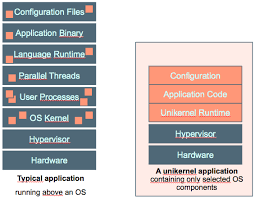
\includegraphics[scale=1]{figures/unikernel_vs_os.png}
\caption{Unikerne vs OS software stack\label{fig3_1}}
\end{figure}

Με λίγα λόγια ένας unikernel αποτελείται από τον κώδικα της εφαρμογής την οποία
θα εκτελέσει, τα απαραίτητα κομμάτια του λειτουργικού συστήματος που η
συγκεκριμένη εφαρμογή χρειάζεται και τις κατάλληλες παραμετροποιήσεις. Τα
unikernels δεδομένου ότι αφορούν μία και μόνο εφαρμογή δεν υποστηρίζουν
περισσότερες από μία διεργασίες, ούτε περισσότερους από έναν χρήστες. Αυτόματα
όλο το κομμάτι των συμβατικών λειτουργικών συστημάτων που αφορούν τη διαχείρηση
και υποστήριξη πολλών διεργασίων και χρηστών καθίσταται άχρηστο και δεν
συμπεριλαμβάνεται. Τα πράγματα είναι διαφορετικά όσον αφορά τα νήματα, καθώς
άλλα unikernel frameworks τα υποστηρίζουν ενώ άλλα όχι. 

Στην εικόνα ~\ref{fig3_1} φαίνεται η διαφορά μεταξύ ενός συμβατικού λειτουργικού
συστήματος και ενός unikernel. Τα παραπάνω ενοποιούνται σε μία εικόνα μηχανής
που μπορεί να εκτελεστεί από έναν επόπτη. Γίνεται εύκολα αντιληπτό ότι το
μέγεθος της τελικής εικόνας θα είναι πολύ μικρότερο από αυτή ενός συμβατικού
λειτουργικού συστήματος. Μία ακόμη συνέπεια αυτού είναι ότι οι χρόνοι εκκίνησης
θα είναι αρκετά μικρότεροι, αφού πλέον δε χρειάζεται να φορτωθούν και να
εκκινήσουν όλες οι υπηρεσίες που προσφέρει ένα λειτουργικό σύστημα. 

Από άποψη ασφάλειας, ο σχεδιασμός των unikernels από μόνος του προσφέρει
σημαντική ασφάλεια. Αρχικά το μικρό μέγεθος των unikernels συνεπάγεται αυτόματα
και μικρότερο εύρος επίθεσης από κάποιον κακόβουλο χρήστη. Επιπλέον πρόκειται
για εξειδικευμένες εικόνες που αφορούν μία και μόνο εφαρμογή, οπότε στην
περίπτωση που αποκτηθεί πρόσβαση στην εικονική μηχανή, το περιθώριο
εκμετάλλευσης θα είναι αρκετά μικρό. Τέλος, υπάρχει απομόνωση μεταξύ των
εικονικών μηχανών η οποία προσφέρεται από τον επόπτη. 

H έλλειψη διαχωρισμού kernelspace και userspace, μειώνει το κόστος
μετάβασης από τον ένα χώρο διευθύνσεων στον άλλο, κάνοντας έτσι τις κλήσεις
συστήματος να λειτουργούν σαν απλές κλήσεις συναρτήσεων. Ως αποτέλεσμα, η
ταχύτητα εκτέλεσης αυξάνει σημαντικά, καθώς δε χρειάζονται πλέον οι μεταβάσεις
από τον ένα χώρο διευθύνσεων στον άλλο, μία αρκετά δαπανηρή λειτουργία.
%% Από την άλλη τίθεται το ζήτημα της ασφάλειας 
%% grapse kati egia auto...

Η έννοια των library operating systems δεν είναι καινούρια, ωστόσο δεν μπορούσαν
να χρησιμοποιηθούν λόγω του μεγάλου πλήθους των συσκευών και συνεπώς των drivers
που θα έπρεπε να υποστηρίζουν. Στις μέρες μας όμως, οι επόπτες έχουν περιορίσει
σημαντικά το πλήθος των συσκευών κάνοντας εφικτή τη χρήση των συγκεκριμένων
λειτουργικών συστημάτων. 
 
Αφ' ετέρου η απομάκρυνση όλων αυτών των υπηρεσιών από το λειτουργικό σύστημα,
δημιουργεί αρκετούς περιορισμούς. Οι περισσότερες εφαρμογές έχουν φτιαχτεί για
συμβατικά λειτυργικά συστήματα λαμβάνοντας υπόψιν και χρησιμοποιοώντας τις
συγκεκριμένες υπηρεσίες. Απαιτείται, λοιπόν, να γίνουν σημαντικές αλλαγές στις
εφαρμογές για να μπορέσουν να εκτελεστούν σε unikernels. Επιπλέον γίνεται πιο
δύσκολη η αποσφαλμάτωση των unikernels δεδομένου των λίγοστών υπηρεσιών που
προσφέρουν. 

\section{Rumprun}
Το rumprun είναι ένα unikernel framework, το οποίο έχει χτιστεί με βάση τα
συστατικά των drivers που προσφέρουν οι rump kernels. 
To rumprun μπορεί να προσφέρει ένα POSIX-like περιβάλλον, το οποίο μπορεί να
χρησιμοποιηθεί από POSIX εφαρμογές ώστε να μετατραπούν χωρίς καμία αλλαγή σε
unikernel εικόνες. Αυτός ήταν και ένας από τους βασικούς στόχους του
εγχειρήματος, η δυνατότητα δηλαδή σε POSIX κώδικα να μπορεί να εκτελεστεί χωρίς
να υποστεί καμία αλλαγή. Στην εικόνα \ref{fig3_2} φαίνεται η δομή του rumprun
για POSIX εφαρμογές (αριστερά) και προσαρμοσμένες εφαρμογές (δεξιά). Προφανώς το
δεξί μοντέλο φαίνεται αρκετά μικρότερο, αλλά είναι απαραίτητες να γίνουν
συγκεκριμένες αλλαγές στην εφαρμογή. O συγκεκριμένος unikernel μπορεί να
εκτελεστεί χρησιμοποιώντας Xen ή KVM, ενώ υποστηρίζει arm και x86
αρχιτεκτονικές. Ο κώδικας του rumprun είναι διαθέσιμος στο
\url{http://repo.rumpkernel.org/rumprun}. 

\begin{figure}[htp]
\centering
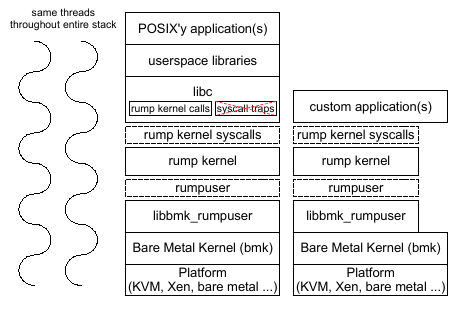
\includegraphics[scale=0.75]{figures/rumprun_stack.png}
\caption{Rumprun software stack\label{fig3_2}}
\end{figure}

Όπως κάθε unikernel framework το rumprun υποστηρίζει μία και μόνο διεργασία.
Μολαταύτα υποστηρίζει POSIX threads, δίνοντας τη δυνατότητα για την ύπαρξη
περισσοτέρων από ένα νήματα. Μάλιστα ο χρονοδρομολογητής που διαθέτει είναι
cooperative, οπότε αν ένα νήμα αποκτήσει τον έλεγχο δνε πρόκειται να διακοπεί
από το χρονδορομοληγτή αλλά θα αφήσει το έλεγχο όταν εκείνο τερματίσει ή
πρόκειται να μπλοκάρει. Κάποιοι ακόμα περιορισμοί, είναι η μη υποστήριξη
εικονικής μνήμης (virtual memory) και σημάτων (signals), Συνεπώς εφαρμογές που
χρησιμοποιούν σήματα ή κλήσεις συστήματος όπως η mmap() δε θα λειτουργούν χωρίς αλλαγές στον κώδικα τους.

Ένας rumprun unikernel αποτελείται από τα απαραίτητα κομμάτια των rump kernels
που χρειάζεται η εφαρμογή και την ίδια την εφαρμογή. Για τη δημιουργία του
unikernel γίνεται πάντα cross-compilation, οπότε δε χρειάζεται κάποιος ήδη
´ετοιμος rumprun unikernels, αλλά μία σειρά από εργαλεία. H διαδικασία έχει ως
εξής:
\begin{enumerate}
	\item Αρχικά γίνεται η μεταγλώττιση του κώδικα της εφαρμογής
		χρησιμοποιοώντας έναν cross-compiler.
	\item Ύστερα, αντί για linking γίνεται pseudo-linking όπως ονομάζουν τη
		διαδικασία κατά την οποία απλά ελέγχονται αν ικανοποιούνται όλες
		οι εξαρτήσεις συμβόλων, χωρίς να γίνεται κάποια σύνδεση με
		κάποιο συστατικό του λειτουργικού συστήματος.
	\item Τέλος, το παράγωγο του προηγούμενου βήματος γίνεται "bake", όπου
		εισάγονται και τα κομμάτια του λειτουργικού συστήματος που
		απαιτούνται, όπως έχουν οριστεί κατά την εκτέλεση της εντολής.
\end{enumerate}

Όπως έχει αναφερθεί ο rumprun unikernel βασίζεται στα rump kernels
~\cite{rumprun_Xen}. Τα rump kernels παρέχουν drivers του NetBSD ως φορητά
εξαρτήματα με τα οποία μπορείς να εκτελέσεις εφαρμογές χωρίς να ναι απαραίτητη η
ύπαρξη λειτουργικού συστήματος ~\cite{kantee2014rump}. Η αρχική ιδέα ήταν να
υπάρχει η δυνατότητα να εκτελούνται αμετάβλητοι drivers του NetBSD ως απλά
προγράμματα σε userspace, ώστε να είναι πιο εύκολος ο έλεγχος και η ανάπτυξη
NetBSD drivers. Ένας rump kernel είναι ένας πυρήνας χρονομερισμού (timesharing)
από τον οποίο έχουν αφαιρεθεί ορισμένα κομμάτια ~\cite{kantee2012design}. Τα
κομμάτια που κρατήθηκαν είναι οι drivers και οι απαραίτητες ρουτίνες που
χρειάζονται οι συγκεκριμένοι drivers για να λειτουργήσουν (συχχρονισμός,
κατανομή μνήμης κ.λ.π.). Τα κομμάτια που αφαιρέθηκαν είναι αυτά που αφορούν τις
διεργασίες, την εικονική μνήμη κ.α.. Επιπλέον τα rump kernels έχουν και ένα
καλώς ορισμένο στρώμα φορητότητας, ώστε να είναι εύκολο να ενσωματωθούν σε
διάφορα περιβάλλοντα.

Πίσω από τα rump kernels υπάρχει μία ακόμα έννοια αυτή του
anykernel ~\cite{kantee2012design}. O συγκεκριμένος όρος δημιουργήθηκε
ως απάντηση στην όλο και αυξανόμενο αριθμό μοντέλων λειτουργικών συστημάτων
(monolithic, exokernel, mikrokernel, unikernel κ.λ.π.). Ένα πολύ μεγάλο ποσοστό
ενός λειτουργικού συστήματος ανεξάρτητα από το μοντέλο που χρησιμοποιεί
αποτελείται από drivers. Ο όρος anykernel περιγράφει ένα κώδικα βάσης (codebase)
τύπου κώδικα πυρήνα από τον οποίο οι οδηγοί μπορούν να εξαχθούν και να
ενσωματωθούν σε οποιοδήποτε μοντέλο λειτουργικού συστήματος, χωρίς να
χρειάζονται αλλαγές και συντήρηση. Στην εικόνα ~\ref{fig3_3} φαίνεται η σχέση
μεταξύ των εννοιών anykernel, rump kernels και rumprun. 


\begin{figure}[htp]
\centering
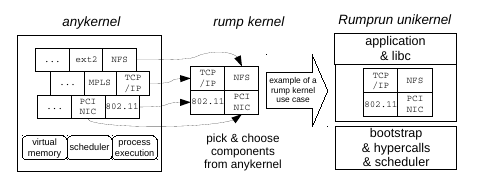
\includegraphics[scale=0.8]{figures/from_anykernel_to_rump.png}
\caption{Σχέση μεταξύ των ενοιών anykernel, rump kernel και rumprun\label{fig3_3}}
\end{figure}

\section{OSv}
dsfdsgfdsgdfs

\section{Click OS}
dsfdsgfdsgdfs

\section{Lkl}
dsfdsgfdsgdfs

\section{Include OS}
dsfdsgfdsgdfs

\section{Mirage OS}
dsfdsgfdsgdfs




\chapter{Σχεδιασμός και υλοποίηση}
\label{chap:implementation}

Όπως είδαμε στο προηγούμενο κεφάλαιο κανένα unikernel framework δεν υποστηρίζει
την κλήση συστήματος fork και επομένως εφαρμογές που χρησιμοποιούν τη
συγκεκριμένη κλήση δεν μπορούν να υποστηριχτούν από αυτά. Στο πλαίσιο, λοιπόν,
της παρούσας διπλωματικής εργασίας δημιουργήσαμε ένα μηχανισμό που
υλοποιεί τις κλήσεις συστήματος fork και pipe σε KVM hypervisor. Ο στόχος ήταν
να διατηρηθεί το single proccess χαρακτηριστικό των unikernels. Για το λόγο
αυτό το αποτέλεσμα της κλησης fork, δεν είναι η δημιουργία μία νέας διεργασίας
στο υπάρχον unikernel, αλλά η εκκίνηση ενός unikernel, ίδιου με το αρχικό. 

Επιπλέον, υλοποιήθηκε και ένας inter-vm communication μηχανισμός, στα πρότυπα
της κλήσης συστήματος pipe. Δηλαδή δύο εικονικά μηχανήματα μπορούν να
επικοινωνούν μεταξύ τους, όπως δύο διεργασίες επικοινωνούν μεταξύ τους, μέσω της
κλήσης συστήματος pipe, σε ένα λειτουργικό σύστημα γενικού σκοπού. 

Στο παρών κεφάλαιο περιγράφουμε αναλυτικά τους δύο αυτούς μηχανισμούς. Το
κεφάλαιο χωρίζεται σε δύο μέρη, ένα για το μηχανισμό pipe και ένα για το
μηχανισμό fork. Σε κάθε μέρος περιγράφεται αναλυτικά τόσο ο μηχανισμός, όσο και
η διαδικασία και τα στάδια μέχρι την τελική υλοποίηση τους.

\newpage
\section{Μηχανισμός pipe}

Σύμφωνα με το POSIX ο ορισμός της κλήσης συστήματος pipe έχει ως εξής:
\begin{lstlisting}[numbers=none,  xleftmargin=.2\textwidth, xrightmargin=.2\textwidth]
int pipe(int fildes[2]);
\end{lstlisting}
Ο μηχανισμός pipe που υλοποιήθηκε που υλοποιήθηκε ακολουθεί τον ορισμό του
POSIX. Πιο συγκεκριμένα μία κλήση στη συγκεκριμένη συνάρτηση δημιουργεί ένα pipe
μεταξύ των δύο εικονικών μηχανημάτων και δημιουργεί δύο νέους file descriptors.
Οι δύο αυτοι file descriptors αποθηκεύονται στις παραμέτρους fildes[0] και
fildes[1]. Ο πρώτος file descriptor αφορά το read κομμάτι του pipe, ενώ ο
δεύτερος το write κομμάτι του pipe. Η τιμή που επιστρέφει η κλήση συστήματος
είναι 0, αν η δημιουργία του pipe ήταν επιτυχής, ενώ διαφορετικά θα επιστραφεί
-1 και η μεταβλητή errno περιέχει την τιμή του σφάλματος.

Η ανάγνωση από το pipe γίνεται χρησιμοποιώντας τον πρώτο file descriptor από τις
παραμέτρους της κλήσης. Τα δεδομένα διαβάζονται με FIFO (first in first out)
σειρά. Ενώ αν δεν υπάρχουν δεδομένα στο pipe τότε η κλήση "μπλοκάρει" μέχρι να
προκύψουν δεδομένα από το write άκρο του pipe. Η εγγραφή στο pipe γίνεται
χρησιμοποιώντας το δεύτερο file descriptor από τις παραμέτρους της κλήσης. Η
εγγραφή στο pipe μπορεί να μπλοκάρει αν δεν υπάρχει χώρος στο pipe. Επιπλέον
μπορεί να αποτύχει αν όλα τα file descriptos για ανάγνωση από το pipe έχουν
κλείσει με το σφάλμα EPIPE. 

\subsection{Στάδια υλοποίησης}

Η υλοποίηση του συγκεκριμένου μηχανσιμού έγινε σε 3 στάδια, τα οποία αναλύονται
παρακάτω. 

\subsubsection{Στάδιο 1 - επίπεδο εφαρμογής}

%%Στο πρώτο στάδιο, δημιουργήσαμε μία επικοινωνία μεταξύ των unikernels,
%%χρησιμοποιώντας TCP/IP sockets. Όπως φαίνεται στην παρακάτω εικόνα \ref{fig4_1}
%%όλη η εργασία για τη δημιουργία της επικοινωνίας γινόταν μέσα από την  εφαρμγοή
%%που εκτελούνταν στο unikernel. Δεδομένου της χρήσης των sockets, κάποιο
%%unikernel θα έπρεπε να είχε το ρόλο του server και το άλλο το ρόλο του client.
%%Όπως γίνεται εύκολα κατανοητό, ο συγκεκριμένος μηχανισμός απαιτεί την ύπαρξη
%%σύνδεσης σε κάποιο κοινό δίκτυο για τα δύο εικονικα μηχανήματα.

Στο πρώτο στάδιο, υλοποιήσαμε το pipe ως μία συνάρτηση που καλείται από την
εφαμρογή. Η συνάρτηση αυτή χρησιμοποιεί TCP/IP sockets για να εγκαθιδρύσει την
επικοινωνία μεταξύ ρων δύο εφαρμογών. Συγκεκριμένα χρησιμοποιούνται δύο sockets,
ένα για την αποστολή δεδομένων και ένα για την παραλαβή. Οι file descriptors των
των δύο αυτών sockets, είναι και οι τιμές που αποθηκεύονται στις μεταβλητές
fildes[0] και fildes[1]. Στην παρακάτω εικόνα \ref{fig4_1} φαίνεται σχηματικά η
υλοποίηση.

\begin{figure}[htp]
\centering
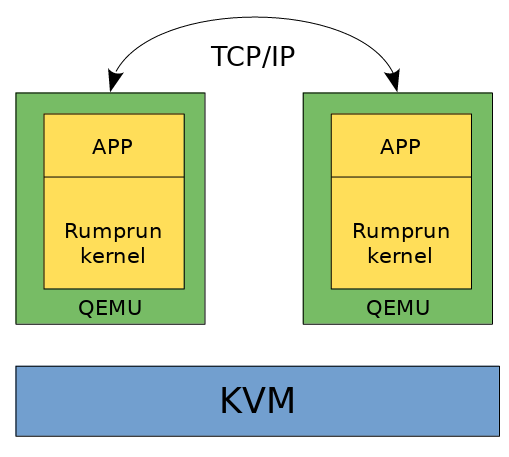
\includegraphics[scale=0.7]{figures/pipe_stage1_function.png}
\caption{Πρώτο στάδιο υλοποίησης μηχανισμού pipe\label{fig4_1}}
\end{figure}

Όπως γίνεται εύκολα κατανοητό η συγκεκριμένη υλοποίηση απαιτεί την ύπαρξη
δικτύου ανάμεσα στα δύο εικονικά μηχανήματα. Επιπλέον, λόγω της χρήσης των
sockets, δεν υλοποιήθηκε όλα τα semantics του pipe. Έτσι ακόμα και αν δεν
υπάρχει ανοιχτό read άκρο στο pipe, οποιαδήποτε εγγραφή στο pipe θα είναι
επιτυχής. Ακόμα, οποιαδήποτε εγγραφή μπορεί να μπλοκάρει μόνο αν ο παραλήπτης
δεν μπορεί να δεχτεί άλλα δεδομένα. Αντιθέτως τα semantics του άκρου ανάγνωσης
του pipe διατηρήθηκαν καθώς και στην περίπτωση των sockets, αν δεν υπάρχουν
δεδομένα προς ανάγνωση η αντίστοιχη κλήση "μπλοκάρει". 

Για να υλοποιηθεί η συνάρτηση pipe, ακολουθήθηκε η ίδια διαδικασία που
ακολουθείται από μία εφαρμογή για να επικοινωνήσει με κάποια άλλη μέσω δικτύου.
Η διαφορά είναι ότι η εφαρμογή έχει το ρόλο του server και του client
ταυτόχρονα. Για αυτό το λόγο χρησιμοποιήθηκαν δύο sockets, ένα για κάθε ρόλο. 
Στην παρακάτω εικόνα \ref{fig4_2} φαίνεται η αλληλουχία κλήσεων συστήματος για
την εγκαθίδρυση της επικοινωνίας (server/client). 

%%O συγκεκριμένος μηχανισμός επικοινωνίας είναι ακριβώς ίδιος με αυτό που
%%χρησιμοποιούν δύο εφαρμογές για να επικοινωνήσουν μεταξύ τους. Ο τρόπος με τον
%%οποίο δημιουργείται ο μηχανισμός με τις ανάλογες κλήσεις συστήματος φαίνεται
%%στην εικόνα \ref{fig4_2}. Όπως φαίνεται από τη μεριά του o client χρειάζεται να
%%ανοίξει ένα socket, να συνδεθεί με το server χρησιμοποιώντας την connect(). Από
%%τη δικιά του μεριά ο server, μετά τη δημιουργία του socket το δεσμεύει σε μία
%%συγκεκριμένη θύρα χρησιμοποιώντας την bind, θέτει το συγκεκριμένο socket ως
%%passive socket ώστε να δεχτεί νέες συνδέσεις με τη listen() και περιμένει κάποια
%%νέα σύνδεση μπλοκάροντας στην accept(). Το συγκεκριμένο στάδιο αποσκοπούσε
%%κυρίως στην περαιτέρω εξοικείωση με το rumprun unikernel framework. Στη συνέχεια
%%η ενδοεπικοινωνία γινόταν γράφοντας και διαβάζοντας στα file descriptors που
%%είχαν δημιουργηθεί από την παραπάνω διαδικασία. 

\begin{figure}[htp]
\centering
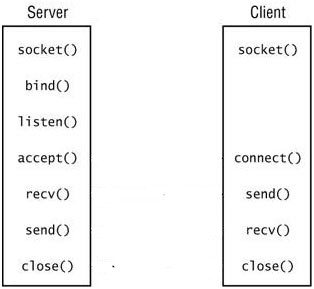
\includegraphics[scale=0.7]{figures/Server_client_syscalls_tcp_ip_socket.jpg}
\caption{Αλληλουχία κλήσεων για επικοινωνία μέσω TCP/IP sockets \label{fig4_2}}
\end{figure}

Η συνάρτηση pipe, λοιπόν ακολουθεί και τις δύο διαδικασίες που φαίνονται
(server/client). Αυτό όμως προξενεί ένα πρόβλημα κατά τη δημιουργία της
επικοινωνίας. Αν και οι δύο εφαρμογές ακολουθήσουν την παραπάνω ακολουθία
κλήσεων τότε θα δημιουργηθεί αδιέξοδο, καθώς και οι 2 θα έχουν κολλήσει στην
κλήση accept, περιμένοντας κάποια σύνδεση. Ο τρόπος με τον οποίο επιλύθηκε το
παραπάνω πρόβλημα είναι ως εξής. Μία από τις δύο εφαρμογές να εκτελεί πρώτα τις
κλήσεις που αφορούν το client κομμάτι και μετά αυτές που αφορούν το server.
Αντίθετα η άλλη εφαρμογή, πρώτα εκτελεί τις κλήσεις που αφορούν το server και
ύστερα αυτές που αφορούν το client μερος. 

\subsubsection{Στάδιο 2 - pipe ως system call με UDP sockets}

Στο δεύτερο στάδιο, υλοποιήσαμε το μηχανισμό του pipe μέσα στον πυρήνα του
rumprun. Ουσιαστικά μετατρέψαμε το function call του προηγούμενου σταδίου σε
system call. Σε αντίθεση με πριν, η επικοινωνία γίνεται μέσω UDP sockets, οπότε
και είναι απαραίτητη η ύπαρξη δικτύου. Η επιλογή του πρωτοκόλλου UDP έναντι του
TCP, έγινε για την πιο εύκολη δημιουργία και χρήση sockets στον πυρήνα του
rumprun. Ο συγκεκριμένος μηχανισμός δίνει τη δυνατότητα να υπάρχει επικοινωνία
μεταξύ δύο ξεχωριστών unikernels, ακόμα και αν αυτά δε μοιράζονται τον ίδιο
host, μέσω μίας κλήσης συστήματος παρόμοια με την pipe(). Με αυτό τον τρόπο, οι
εφαρμογές δε χρειάζονται να τροποποιηθούν σε μεγάλο βαθμό, από την αρχική τους
έκδοση. Στην παρακάτω εικόνα ~\ref{fig4_3} φαίνεται σχηματικά η υλοποίηση.

\begin{figure}[htp]
\centering
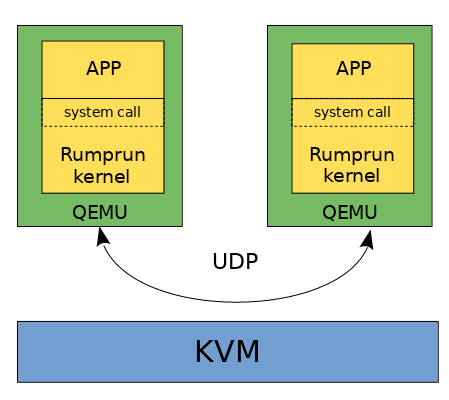
\includegraphics[scale=0.7]{figures/pipe_stage2.png}
\caption{Δεύτερο στάδιο υλοποίησης μηχανισμού pipe\label{fig4_3}}
\end{figure}

Όσον αφορά τη χρήση του μηχανισμού, αυτή γίνεται ακολουθώντας την ίδια
διαδικασία με τη χρήση της κλήσης pipe σε ένα UNIX σύστημα. Στις παραμέτρους
fildes[0], fildes[1], αποθηκεύονται οι δύο file descriptors που θα
χρησιμοποιηθούν για την ανάγνωση και εγγραφή αντίστοιχα. Σε περίπτωση επιτυχίας
επιστρέφεται η τιμή 0, ενώ σε αντίθετη περίπτωση, στη μεταβλητή errno
αποθηκεύεται ο κωδικός του σφάλματος. Δεδομένου, ότι η επικοινωνία γίνεται με
UDP sockets, τα semantics είναι ίδια με το προηγούμενο στάδιο. Μία σημαντική
διαφορά, είναι ότι πρέπει να καθοριστεί η διεύθυνση IP του unikernel με το οποίο
θα εγκαθιδρυθεί η επικοινωνία. Για το λόγο αυτό, μετά την κλήση της pipe() θα
πρέπει μέσω της ioctl στο file descriptor της εγγραφής 
\begin{lstlisting}[numbers=none,  xleftmargin=.05\textwidth, xrightmargin=.05\textwidth]
ioctl(fildes[1], SETIPADDR, htonl(IP_ADDRESS));
\end{lstlisting}
Η μορφή της IP διεύθυνσης θα πρέπει να είναι σε network byte order
και για αυτό το σκοπό μπορεί να χρησιμοποιηθεί η συνάρτηση htonl.
Ο τρόπος που λειτουργεί ο μηχανισμός έχει ως εξής:
\begin{enumerate}
	\item Αρχικά καλώντας την pipe, επιστρέφονται τα δύο απαραίτητα file
		descriptors, ένα για εγγραφή και ένα για ανάγνωση.
	\item Στη συνέχεια, πρεπει να οριστεί η διεύθυνση IP, στην οποία θέλουμε
		να στείλουμε τα δεδομένα. Αυτό γίνεται μέσω της προαναφερθείσας
		ioctl κλήσης. 
	\item Η εφαρμογή στέλνει δεδομένα χρησιμοποιώντας την κλήση write() και
		το file descriptor που αντιπροσωπεύει το άκρο εγγραφής του pipe.
	\item H εφαρμογή λαμβάνει δεδομένα χρησιμοποιώντας την κλήση read() και
		το file descriptor που αντιπροσωπεύει το άκρο ανάγνωσης του pipe.
\end{enumerate}

Η μεταφορά του μηχανισμού στον πυρήνα του rumprun απαιτούσε και τις ανάλογες
αλλαγές στις συναρτήσεις που χρησιμοποιήθηκαν, καθώς πλέον ο προγραμματισμός
γινόταν εντός του πυρήνα. Ο πυρήνας που χρησιμοποιεί το rumprun είναι αυτός του
NetBSD και σε σχέση με τον τρόπο που χρησιμοποιούνται τα sockets σε userspace,
διαφέρει με τον αντίστοιχο σε kernelspace. Ο συγκεκριμένος μηχανισμός
χρησιμοποιεί ένα struct, στο οποίο αποθηκεύονται το socket, το file descriptor
και η διεύθυνση IP του παραλήπτη. 
\begin{lstlisting}[numbers=none,  xleftmargin=.2\textwidth, xrightmargin=.2\textwidth]
struct pipe_data {
	struct socket *so;
	uint32_t ip;
	int fd;
};
\end{lstlisting}
Παρακάτω, περιγράφεται τι γίνεται μέσα στον πυρήνα όταν εκτελούνται οι παραπάνω
κλήσεις. 
\begin{enumerate}
	\item pipe: Αρχικά, δημιουργούνται δύο sockets με την socreate, ένα για
		αποστολή και ένα για παραλαβή δεδομένων και αποθηκεύονται στα
		αντίστοιχα πεδία του struct pipe\_data. Το socket που θα
		χρησιμοποιηθεί για ανάγνωση γίνεται bind στη θύρα 23456 με την
		sobind,	επιτρέποντας συνδέσεις από κάθε IP. Στη συνέχεια,
		δημιουργούνται τα 2 file descriptors που θα χρησιμοποιούνται από
		την εφαρμογή. Τα file descriptos, από τη μεριά του πυρήνα
		αντιπροσωπεύονται από τις δομές file\_t. Στις δομές
		αυτές αποθηκεύεται και το struct pipe\_data που αναφέρθηκε
		προηγουμένως. Αν όλα έχουν πάει καλά, προστίθονται τα δύο file
		descriptors στην εφαρμογή και επιστρέφει με επιτυχία η pipe.
	\item ioctl: Όταν καλείται η ioctl με το command SETIPADDR, αποθηκεύεται
		στο πεδίο ip του pipe\_data η τιμή που έχει περαστεί ως τρίτη
		παράμετρος στην ioctl.
	\item write: Αρχικά αρχικοποιείται το struct sockaddr\_in, το οποίο
		λαμβάνει την IP του παραλήπτη από το πεδίο ip του pipe\_data.
		Στη συνέχεια χρησιμοποιώντας τη sosend, στέλνονται τα δεδομένα
		μέσα από το socket.
	\item read: Με τη χρήση της soreceive, διαβάζονται τυχόν δεδομένα στο
		socket. Αν δεν υπάρχουν δεδομένα η soreceive μπλοκάρει μέχρι να
		προκύψουν.
\end{enumerate}

Στον πυρήνα του NetBSD, τυχόν δεδομένα που μεταφέρονται από userspace σε
kernelspace αποθηκεύονται στο struct uio. Τόσο η soreceive, όσο και η sosend,
δίνουν τη δυνατότητα να χρησιμοποιηθεί το συγκεκριμένο struct και συνεπώς δεν
υπάρχει ανάγκη για παραπάνω αντιγραφές των δεδομένων. Η διαδικασία για την
εισαγωγή μία νέας κλήσης συστήματος στο rumprun, είναι ακριβώς ίδια με αυτή που
θα χρησιμοποιηθεί για την εισαγωγή μία κλήσης συστήματος στον πυρήνα του NetBSD,
με ένα επιπλέον βήμα. Αφού εισαχθεί η κλήση συστήματος στο NetBSD, πρέπει να
εισαχθεί στο αρχείο src-netbsd/sys/rump/librump/rumpkern η κλήση συστήματος.
Σε αυτό το σημείο, καλό είναι να ξανααναφερθεί ότι στα unikernels δεν υπάρχει
διαχωρισμός μεταξύ userspace και kernelspace, ωστόσο οι συγκεκριμένοι όροι
χρησιμοποιούνται για να γίνει διαχωρισμός μεταξύ του κώδικα μίας οποιασδήποτε
εφαρμογής και του κώδικα του πυρήνα του unikernel.

%% -----------------------------------------------------------------------------
%% ------------------------ Deutero stadio me device ---------------------------
%% -----------------------------------------------------------------------------

%%Στο δεύτερο στάδιο, υλοποιήσαμε το μηχανισμό, μέσα στον πυρήνα του rumprun. Όπως
%%και στο προηγούμενο στάδιο, έτσι και εδώ η επικοινωνία γίνεται μέσψ TCP/IP
%%sockets, συνεπώς είναι απαραίτητη η ύπαρξη δικτύου. Βέβαια ο συγκεκριμένος
%%μηχανισμός μπορεί να χρησιμοποιηθεί για την επικοινωνία rumprun unikernels που
%%δε βρίσκονται στον ίδιο host. Ο τρόπος με τον οποίο επιλέχθηκε να γίνει αυτό
%%είναι μέσω μίας ψευδοσυσκευής. Στην παρακάτω εικόνα \ref{fig4_3} φαίνεται 
%%σχηματικά η υλοποίηση.  
%%
%%\begin{figure}[htp]
%%\centering
%%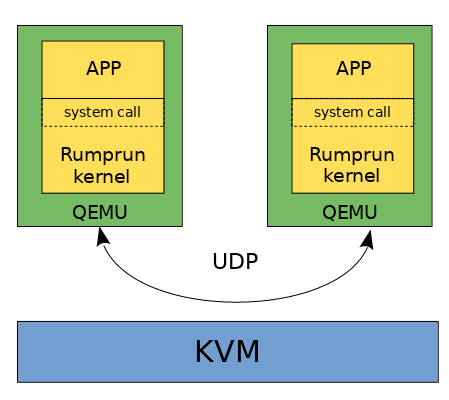
\includegraphics[scale=0.7]{figures/pipe_stage2.png}
%%\caption{Δεύτερο στάδιο υλοποίησης μηχανισμού pipe\label{fig4_3}}
%%\end{figure}
%%
%%Στο επίπεδο της εφαρμογής, ο μηχανισμός είναι διαθέσιμος μέσω της συσκευής
%%/dev/comso. Ανοίγωντας τη συγκεκριμένη συσκευή, η εφαρμογή έχει τη δυνατότητα να
%%στέλνει και να λαμβάνει δεδομένα, γράφοντας και διαβάζοντας αντίστοιχα στη
%%συγκεκριμένη συσκευή. Ουσιαστικά το pipe έχει μετατραπεί σε μία ψευδοσυσκευή που
%%μπορεί να επικοινωνήσει μέσω TCP/IP sockets, με άλλες εφαρμογές. Ο τρόπος με τον
%%οποίο υλοποιήθηκε ο μηχανισμός, αλλάζει τον ορισμό του pipe, καθώς μέσω του
%%ίδιου file descriptor, η εφαρμογή μπορεί να γράψει ή να διαβάσει δεδομένα. Τέλος
%%τα semantics είναι ίδια με το προηγούμενο στάδιο. 
%%
%%Η μεταφορά του μηχανισμού στον πυρήνα του rumprun απαιτούσε και τις ανάλογες
%%αλλαγές στις συναρτήσεις που χρησιμοποιήθηκαν, καθώς πλέον ο προγραμματισμός
%%γινόταν εντός του πυρήνα. Ο πυρήνας που χρησιμοποιεί το rumprun είναι αυτός του
%%NetBSD και σε σχέση με τον τρόπο  που χρησιμοποιούνται τα sockets σε userspace,
%%διαφέρει με τον αντίστοιχο σε kernelspace. Ο τρόπος που λειτουργεί ο μηχανισμός
%%φαίνεται στην εικόνα \ref{fig4_4} και μία σύντομη περιγραφή του έχει ως εξής:
%%\begin{enumerate}
%%	\item Αρχικά η εφαρμογή χεησιμοποιεί την open για να ανοίξει τη συσκευή.
%%		Από τη μεριά του πυρήνα, αυτό έχει ως αποτέλεσμα τη δημιουργία
%%		του socket που θα χρησιμοποιηθεί για την επικοινωνία. Η
%%		δημιουργία του socket γίνεται χρησιμοποιώντας τη sosocket().
%%	\item Η εφαρμογή στέλνει δεδομένα χρησιμοποιώντας την κλήση write() και
%%		το file descriptor που αντιπροσωπεύει την ανοιχτή συσκευή comso.
%%		Από τη μεριά του πυρήνα, όταν λαμβάνεται το συγκεκριμένο αίτημα
%%		χρησιμοπποιείται η sosend, για να σταλούν τα δεδομένα μέσω του
%%		socket στον προορισμό.
%%	\item H εφαμρογή λαμβάνει δεδομένα χρησιμοποιώντας την κλήση open() και
%%		το file descriptor που αντιπροσωπεύει την ανοιχτή συσκευή comso.
%%		Από τη μεριά του πυρήνα, όταν λαμβάνεται το συγκεκριμένο αίτημα
%%		γίνεται bind το socket, σε μία συγκεκριμένη θύρα, με τη sobind,
%%		και στη συνέχεια, χρησιμοποιείται η soreceive. Η συγκεκριμένη
%%		συνάρτηση του πυρήνα του NetBSD περιμένει να υπάρξει μία νέα
%%		σύνδεση και στη συνέχεια περιμένει να λάβει δεδομένα που έχουν
%%		σταλεί στο συγκεκριμένο socket.
%%	\item Τέλος, όταν η εφαρμογή κλείσει το αρχείο που αντιπροσωπεύει την
%%		ψευδοσυσκευή comso μέσω της close, στον πυρήνα αυτό οδηγεί και
%%		στο κλείσιμο του socket, χρησιμοποιώντας τη soclose.
%%\end{enumerate}
%%
%%Στον πυρήνα του NetBSD, τυχόν δεδομένα που μεταφέρονται από userspace σε
%%kernelspace αποθηκεύονται στο struct uio. Τόσο η soreceive, όσο και η sosend,
%%δίνουν τη δυνατότητα να χρησιμοποιηθεί το συγκεκριμένο struct και συνεπώς δεν
%%υπάρχει ανάγκη για παραπάνω αντιγραφές των δεδομένων. Σε αυτό το σημείο, καλό
%%είναι να ξανααναφερθεί ότι στα unikernels δεν υπάρχει διαχωρισμός μεταξύ
%%userspace και kernelspace, ωστόσο οι συγκεκριμένοι όροι χρησιμοποιούνται για να
%%γίνει διαχωρισμός μεταξύ του κώδικα μίας οποιαδήποτε εφαρμογής και του κώδικα
%%του unikernel.
%%
%%\begin{figure}[htp]
%%\centering
%%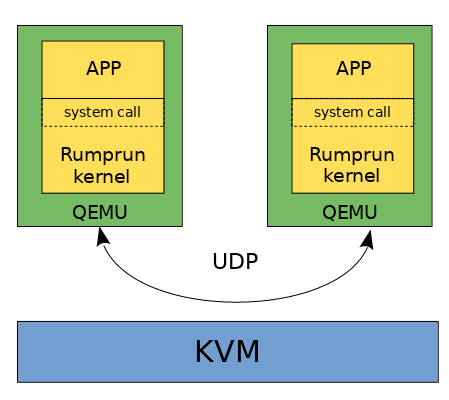
\includegraphics[scale=0.7]{figures/pipe_stage2.png}
%%\caption{Δεύτερο στάδιο υλοποίησης μηχανισμού pipe\label{fig4_3}}
%%\end{figure}
%%------------------------------------------------------------------------------
%%------------------------------------------------------------------------------

\subsubsection{Στάδιο 3 - pipe ως function call με shared memory}

Στο τελευταίο στάδιο, υλοποιήσαμε το μηχανισμό pipe, πάλι ως system call με τη
διαφορά ότι πλέον δε χρησιμοποιούνται sockets, αλλά κοινή μνήμη μεταξύ των
εικονικών μηχανημάτων. Πλέον δεν υπάρχει ανάγκη για ύπαρξη δικτύου μεταξύ των
εικονικών μηχανημάτων, ωστόσο η συγκεκιμένη υλοποίηση μπορεί να χρησιμοποιηθεί
μόνο για unikernels, που μοιράζονται τον ίδιο host. Για την κοινή μνήμη
χρησιμοποιήθηκε το ivshmem \cite{macdonell2011shared}. Όπως έχει ήδη αναφερθεί
πρόκειται για ένα μηχανισμό, που επιτρέεπει το διαμοιρασμό μνήμης μεταξύ του
host και των εικονικών μηχανών που εκτελούνται στο host. Η χρήση του γίνεται
μέσω μίας PCI συσκευής. Συνεπώς έπρεπε να δημιουργήσουμε τον κατάλληλο driver
που θα μας επιστρέψει να το χρησιμοποιήσουμε. Στην παρακάτω εικόνα \ref{fig4_4}
φαίνεται σχηματικά η υλοποίηση. 

\begin{figure}[htp]
\centering
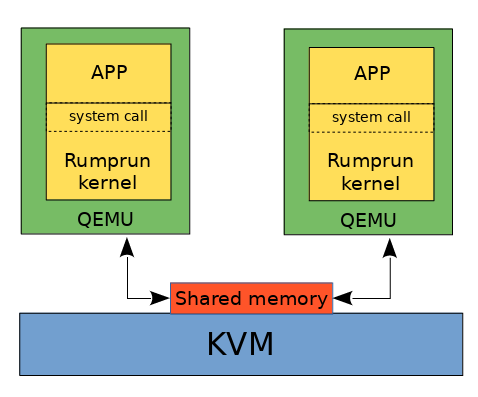
\includegraphics[scale=0.7]{figures/pipe_stage3.png}
\caption{Τρίτο στάδιο υλοποίησης μηχανισμού pipe\label{fig4_4}}
\end{figure}

Η χρήση του pipe, από την εφαρμογή γίνεται πλέον όπως σε κάθε UNIX λειτουργικό
σύστημα. Καλώντας την pipe, αν όλα πάνε καλά αποθηκεύονται στις
παραμέτρους fildes[0], fildes[1], οι δύο file descriptors που θα χρησιμοποιηθούν
για την ανάγνωση και εγγραφή αντίστοιχα. Σε περίπτωση επιτυχίας επιστρέφεται η
τιμή 0, ενώ σε αντίθετη περίπτωση, στη μεταβλητή errno αποθηκεύεται ο κωδικός
του σφάλματος. Επιπλέον έχουν υλοποιηθεί και όσα semantics δεν είχαν υλοποιηθεί
στα προηγούμενα στάδια. Οπότε, σε περίπτωση που δεν υπάρχουν ανοιχτά άκρα
ανάγνωσης στο pipe, η εγγραφή δε θα είναι επιτυχής. Αν δεν υπάρχει αρκετός χώρος
για την εγγραφή δεδομένων, τότε η write "μπλοκάρει".

Θα ξεκινήσουμε την περιγραφή της υλοποίησης από την υλοποίηση του PCI driver για
το ivshmem. Αρχικά πρέπει να ενημερώσουμε το qemu για τη χρήση του συγκεκριμένου
μηχανισμού. Για να γίνει αυτό χρησιμοποιούμε τις ακόλουθες παραμέτρους για το qemu.
\begin{lstlisting}[numbers=none]
-device ivshmem-plain,memdev=hostmem -object memory-backend-file,size=1M,share,mem-path=/dev/shm/ivshmem,id=hostmem
\end{lstlisting}
%% TODO na dw an isxuei auto pou grafw me to mempath
Στην παράμετρο size, ορίζουμε τη χωρητικότητα του pipe και για κάθε pipe πρέπει
να ορίσουμε διαφορετικό mem-path. Κάθε unikernel που ξεκινάει με τις
συγκεκριμένες παραμέτρους μπορεί να χρησιμοποιήσει το pipe. 

Από τη μεριά του unikernel, χρειάζεται να κατασκευάσουμε έναν PCI driver για το
μηχανισμό ivshmem. Όπως και στην περίπτωση του system call έτσι και στην
περίπτωση του driver, αρχικά πρέπει να φτιάξουμε το driver για το NetBSD. 
Ακολουθώντας το Kernel Development Manual του NetBSD ~\cite{NetBSDKDMDriver},
για τον pci device driver υλοποιήσαμε τρεις συναρτήσεις:
\begin{enumerate}
	\item match: Είναι η συνάρτηση που καλείται από το autoconfiguration
		framework του NetBSD, όταν το σύστημα εκκινεί, ώστε να
		ταιριαστεί ο driver με τη συσκευή. Οπότε στην περίπτωση του
		δικού μας driver η συγκεκιμένη συνάρτηση ελέγχει αν πρόκειται
		για ivshmem pci device, ελέγχοντας τις τιμές του κατασκευαστή
		και το id της συσκευής.
	\item attach: Καλείται μόνο αν η ανίσχνευση της συσκευής ήταν επιτυχής
		(αν η match επέστρεψε 1). Ο ρόλος της είναι να αρχιοποιήσει τη
		συκευή. Δεδομένου, ότι εμείς χρησιμοποιούμε το συγκεκριμένο
		μηχανισμό απλά για διαμοιρασμό μνήμης, αρκεί να κάνουμε map το
		PCI\_BAR(2) του ivshmem και να αποθηκεύσουμε τις απαραίτητες
		μεταβλητές για τη χρήση του μηχανισμού.
	\item detach: Καλείται σε περίπτωση που η συσκευή αποσυνδεθεί. Στη δική
		μας περίπτωση είναι αρκετό να κάνουμε unmap το bus\_space που
		χρησιμοποιούμε και να μηδενίσουμε τις μεταβλητές που
		χρησιμοποιούμε για τη συσκευή.
\end{enumerate}

Προκειμένου να μπορεί να χρησιμοποιηθεί η συσκευή από τον υπόλοιπο πυρήνα του
NetBSD, είναι απαραίτητο να αποθηκευτούν οι απαραίτητες μεταβλητές που
αναφέρθηκαν στις συναρτήσεις attach και detach. Για το λόγο αυτό δημιουργήθηκε
το struct ivshm, που έχει ως πεδία τις μεταβλητές αυτές. 
\begin{lstlisting}[numbers=none]
struct ivshm {
	bus_size_t		data_s;	/* size of shared memory */
	bus_addr_t		data_b;	/* base address of shared memory */
	bus_space_tag_t		data_t;	/* bus tag for shared memory */
	bus_space_handle_t	data_h;	/* bus handle for shared memory */
};
\end{lstlisting}
Ιδανικά θα θέλαμε να κάνουμε map όλη την κοινή μνήμη του ivshmem, ώστε να μπορεί
να χρησιμοποιηθεί σαν μνήμη του πυρήνα. Ωστόσο, το rumprun δεν υποστηρίζει το
maping μνήμης μέσω του bus. Ως εκ τούτου, η πρόσβαση στην κοινή μνήμη γίνεται
κάθε φορά με εγγραφή και ανάγνωση bytes από αυτήν χρησιμοποιώντας το bus. Υπό
αυτές τις συνθήκες, υπήρχαν τέσσερις μεταβλητές που ήταν απαραίτητες:
\begin{enumerate}
	\item το μέγεθος της κοινής μνήμης.
	\item η διεύθυνση βάσης της κοινής μνήμης
	\item το bus tag της κοινής μνήμης
	\item και το bus handle της κοινής μνήμης.
\end{enumerate}
Οι 2 τελευταίες μεταβλητές, είναι αυτές που χρησιμοποιούνται από τις συναρτήσεις
που παρέχει το NetBSD για να μπορέσει χρησιμοποιώντας το bus, να επικοινωνήσει
με τη συσκευή. Ο ρόλος των υπόλοιπων δύο μεταβλητών θα γίνει πιο ξεκάθαρος
παρακάτω.

Αφού λοιπόν, δημιουργήσαμε το driver για το NetBSD και ενημερώσαμε το
autoconfiguration framework για την ύπαρξη του, έπρεπε να κάνουμε γνωστή την
ύπαρξη του και στο rumprun. Για να γίνει αυτό απαιτούνται δύο ενέργεις. Πρώτον
προσθέτουμε το pci driver στο src-netbsd/sys/rump/dev/Makefile.rumpdevcomp.
Δεύτερον, να δημιουργηθεί ένα νέο directory στο src-netbsd/sys/rump/dev/lib/ για
τη νέα συσκευή. Το directory υατό περιέχει το ioconf και το απαραίτητο Makefile
για να προστεθεί o οδηγός μας στο build σύστημα του rumprun. 

\begin{lstlisting}[caption={IVSHMEM.ioconf},captionpos=b]
ioconf ivshmem

include "conf/files"
include "dev/pci/files.pci"
include "rump/dev/files.rump"

pseudo-root pci*

ivshmem* at pci? dev ? function ?
\end{lstlisting}

\begin{lstlisting}[caption={rumprun Makefile για το ivshmem},captionpos=b]
RUMPTOP=${TOPRUMP}

.PATH:	${RUMPTOP}/../dev/pci

LIB=	rumpdev_ivshmem
COMMENT=ivshmem

IOCONF=	IVSHMEM.ioconf
RUMP_COMPONENT=ioconf

SRCS+=	ivshmem.c
##SRCS+=	ivshmem_component.c

CPPFLAGS+= -I${RUMPTOP}/librump/rumpkern

.include "${RUMPTOP}/Makefile.rump"
.include <bsd.lib.mk>
.include <bsd.klinks.mk>
\end{lstlisting}

Η αρθρωτή οργάνωση των unikernels, δίνει τη δυνατότητα κάθε φορά να επιλέγονται
μόνο τα απαραίτητα συστατικά για κάθε unikernel. Σε αυτό αποσκοπεί και η
δημιουργία του παραπάνω directory, ώστε να μπορεί ο συγκεκιμένος driver να
ενσωματωθεί στο unikernel, κατά τη διάρκεια του baking. Για τη χρήση του
συγκεκριμένου οδηγού είναι απαραίτητη η εισαγωγή του -lrumpdev\_ivshmem στο
config με το οποίο θα γίνει bake η εφαρμογή. 

Αφού δημιουργήσαμε τον driver, το επόμενο βήμα ήταν η αλλαγή του system call,
ώστε αντί για sockets να χρησιμοποιείται ο μηχανισμός του ivshmem. Αρχικά, δε
χρειαζόμαστε την ioctl κλήση και δημιουργούμε δύο structs, το struct pipe και το
struct pipe\_op. Οι ορισμοί τους φαίνονται παρακάτω:

\begin{lstlisting}
struct pipe {
	bus_size_t	init;		/* is shared memory initalized? */
	bus_size_t	lock;		/* pipe lock */
	bus_size_t	wr_lock;	/* writers lock */
	bus_size_t	nreaders;	/* number of readers in pipe */
	bus_size_t	nwriters;	/* number of writers in pipe */
	bus_size_t	len;		/* size of pipe buffer */
	bus_size_t	in;		/* pointer for next write */
	bus_size_t	out;		/* pointer for next read */
	bus_size_t	cnt;		/* number of bytes in pipe */
	bus_size_t	buf;		/* pipe buffer */
	int		pr_readers;	/* readers from this process */
	int		pr_writers;	/* writers from curr process */
};

struct pipe_op {
	int		oper;		/* operation in pipe 0 for read,
					   1 for write*/
	struct pipe	*pipe;
};
\end{lstlisting}

Το struct pipe\_op συνδέεται με τα file descriptors που δημιουργεί η κλήση pipe,
ένα για κάθε file descriptor. H μεταβλητή oper, καθορίζει αν πρόκειται για το
file descriptor που αφορά την εγγραφή στο pipe ή αυτό που αφορά στην ανάγνωση. η
άλλη τιμή είναι το struct pipe που είναι κοινό και για τα δύο άκρα του pipe και
περιέχει βοηθητικές μεταβλητές για τη διαχείρηση του pipe. Όπως έχει ήδη
αναφερθεί η χρήση της κοινής μνήμης γίνεται μέσω του bus και οι συναρτήσεις
εγγραφής ή ανάγνωσης από το bus απαιτούν ως παράμετρο τη διεύθυνση βάσης από την
οποία θα διαβαστούν τα δεδομένα. Έτσι για να αναφερθούμε σε διαφορετική
μεταβλητή μέσα σε αυτή τη μνήμη θα πρέπει να χρησιμοποιήσουμε διαφορετική
διεύθυνση βάσης. Συνεπώς, το struct pipe περιέχει τις διευθύνσεις των κοινών
μεταβλητών στην κοινή μνήμη. Επιπλέον, χρησιμοποιούνται και οι μεταβλητές
pr\_readers και pr\_writers που αφορούν τα ανοιχτά άκρα στο pipe από τη
συγκεκριμένη διεργασία. Η δύο τελευταίες μεταβλητές είναι απαραίτητες για τη
διαχείρηση του pipe όταν η διεργασία που έχει δημιουργήσει το pipe κάνει fork.

\begin{figure}[htp]
\centering
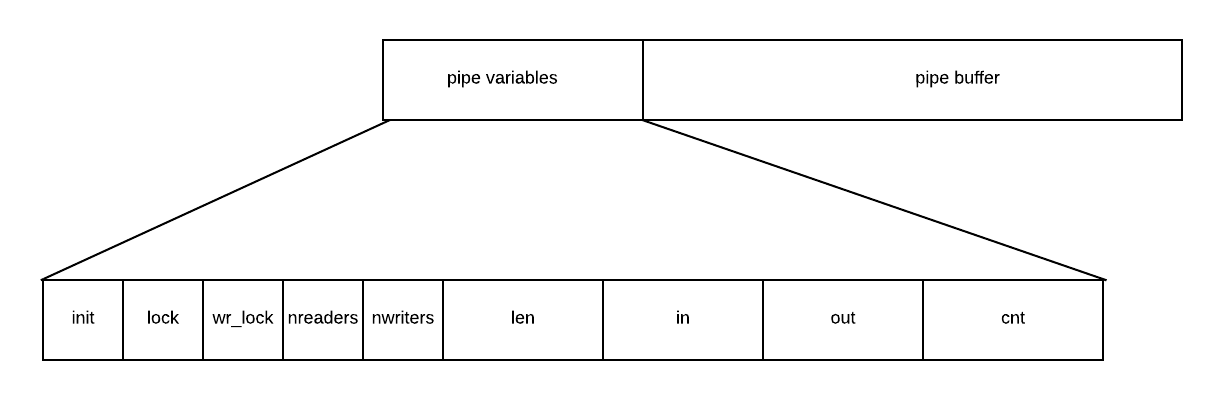
\includegraphics[scale=0.7]{figures/shared_memoery_layout.png}
\caption{shared memory layout\label{fig4_5}}
\end{figure}

Αν θεωρήσουμε την κοινή μνήμη σαν ένα μεγάλο συνεχόμενο κομμάτι μνήμης, τότε
στην παραπάνω εικόνα ~\ref{fig4_5} φαίνεται πως την έχουμε διαχωρίσει εσωτερικά,
με ένα κομμάτι της να αφορά τις μοιραζόμενες μεταβλητές και ένα άλλο τον buffer
του pipe. Οι αρχικές μεταβλητές, έχουν μικρότερο μέγεθος από τις τελευταίες και
η λειτουργία της κάθε μίας έχει ώς εξής:
\begin{itemize}
	\item init: Πρόκειται για μία μεταβλητή ελέγχου, που καθορίζει αν έχουν
		αρχικοποιηθεί οι κοινές μεταβλητές του pipe. Αλλάζεις μόνο δύο
		φορές, όταν πρωτοδημιουργείται το pipe και όταν αυτό
		καταστρέφεται. Ουσιαστικά δηλώνει αν οι υπόλοιπες μεταβλητές
		περιέχουν "σκουπίδια", ή αν έχουν χρήσιμες τιμές.
	\item lock: Πρόκειται για το γενικό lock του pipe και προστατεύει όλες
		τις κοινές μεταβλητές του pipe. 
	\item wr\_lock: Πρόκειται για ένα lock που κάθε φορά επιτρέπει σε ένα
		και μόνο unikernel ννα γράφει στο pipe. 
	\item nreaders: Ο αριθμός των ανοιχτών άκρων ανάγνωσης για το pipe
	\item wreaders: Ο αριθμός των ανοιχτών άκρων εγγραφής για το pipe
	\item len: Το μέγεθος του pipe buffer.
	\item in: Ο δείκτης που καθορίζει σε ποιο σημείο θα γραφτούν τα νέα
		δεδομένα στο pipe buffer.
	\item out: Ο δείτης που καθορίζει από ποιο σημείο θα διβαστούν δεδομένα
		από το pipe buffer
	\item cnt: Μετρητής των bytes που υπάρχουν στο pipe, κάθε στιγμή
\end{itemize}

Για την πρόσβαση στις παραπάνω μεταβλητές και γενικά για την κοινή μνήμη
χρησιμοποιήθηκαν οι συναρτήσεις bus\_space\_read\_1, bus\_space\_read\_4,
bus\_space\_write\_1, bus\_space\_write\_4. Ο αριθμός στο τέλος της κάθε
συνάρτησης υποδηλώνει το μέγεθος των δεδομένων που θα διαβαστούν ή θα γραφτούν.
Για την πιο εύκολη χρήση της κοινής μνήμης δημιουργήθηκαν 4 βοηθητικές
συναρτήσεις, που φαίνονται παρακάτω. 

\begin{lstlisting}
/*
 * Read a region of bytes in bus (data is 1 byte)
 */
void read_region_1(bus_size_t offset, uint8_t *datap, bus_size_t count)
{
	int i;
	for (i=0; i<count; i++) {
		datap[i] = bus_space_read_1(sharme.data_t, sharme.data_h,
				offset + i);
	}
	return;
}

/*
 * Read a region of bytes in bus (data is 4 byte)
 */
void read_region_4(bus_size_t offset, uint32_t *datap, bus_size_t count)
{
	int i;
	for (i=0; i<count; i++) {
		datap[i] = bus_space_read_4(sharme.data_t, sharme.data_h,
				offset + i*4);
	}
	return;
}

/*
 * Write in a region of bytes in bus (data is 1 byte)
 */
void write_region_1(bus_size_t offset, uint8_t *datap, bus_size_t count)
{
	int i;
	for (i=0; i<count; i++) {
		bus_space_write_1(sharme.data_t, sharme.data_h, offset + i,
				datap[i]);
	}
	return;
}

/*
 * Write in a region of bytes in bus (data is 4 byte)
 */
void write_region_4(bus_size_t offset, uint32_t *datap, bus_size_t count)
{
	int i;
	for (i=0; i<count; i++) {
		bus_space_write_4(sharme.data_t, sharme.data_h,	offset + i*4,
				datap[i]);
	}
	return;
}
\end{lstlisting}

Οι παραπάνω συναρτήσεις διαβάζουν ή γράφουν σε μία περιοχή μνήμης, είτε 1 είτε 4
bytes δεδομένα. Το μέγεθος της περιοχής που θα γίνει η πρόσβαση καθορίζεται από
την παράμετρο count και το μέγεθος των bytes (count * bytes\_of\_data). Οι άλλες
2 παράμετροι των συναρτήσεων είναι η διεύθυνση βάσης για το bus και ένας πίνακας
, στον οποίο αποθηκεύονται τα δεδομένα που διαβάστηκαν από μνήμη είτε τα
δεδομένα που θα γραφτούν στην περίπτωση, στις λειτουργίες read και write
αντίστοιχα. Οι συναρτήσεις bus\_space, χρησιμοποιούν τη δομή struct ivshm, για
τις μεταβλητές bus tag και bus handle. Όλες οι αναφορές στην κοινή μνήμη, πέρα
από αυτές των locks, γίνονται χρησιμοποιώντας αυτές τις συναρτήσεις.

Η ύπαρξη κοινής μνήμης μεταξύ διαφορετικών unikernels, απαιτεί και την ύπαρξη
κάποιου συγχρονισμού μεταξύ αυτών. Για αυτό σκοπό χρησιμοποιούνται τα δύο locks
στο struct pipe (lock, wr\_lock). Τα δύο αυτά locks, βρίσκονται εντός της κοινής
μνήμης και απαιτούν ειδική μεταχείριση. Ο μηχανισμός ivshmem μπορεί να
υποστηρίξει τη χρήση ατομικών εντολών του gcc. Για το λόγο, αυτό δημιουργήσαμε
δύο ακόμα συναρτήσεις για το locking, μία για την απόκτηση του κλειδώματος και
μία για την απελευθέρωση του. Ου συναρτήσεις αυτές φαίνονται παρακάτω. 

\begin{lstlisting}
/*
 * Spinlock for pipe
 */
void pipe_lock(bus_size_t lock)
{
	while(__sync_val_compare_and_swap((uint8_t *)sharme.data_b + lock, 0, 1) == 1)
		/* do nothing */;
	return;
}

/*
 * Release the lock
 */
void pipe_unlock(bus_size_t lock)
{
	__sync_lock_release((uint8_t *)sharme.data_b + lock);
	return;
}

\end{lstlisting}

Οι ατομικές εντολές που χρησιμοποιήθηκαν για τη χρήση του lock, είναι οι
\_\_sync\_val\_compare\_and\_swap και \_\_sync\_lock\_release. Οι εντολές αυτές
δέχονται ως παράμετρο τη διεύθυνση της μνήμης στην οποία θα γίνει η πρόσβαση. Η
διεύθυνση αυτή καθορίζεται από τη διεύθυνση βασης των δεδομένων (data\_b) στο
struct ivshmem και το offset του lock μέσα στην κοινή μνήη που είναι
αποθηκευμένο στο struct pipe. Οποιαδήποτε αλλαγή σε κάποιο κομμάτι της κοινή
μνήμης απαιτεί την απόκτηση του γενικού lock, ενώ οποιαδήποτε εγγραφή στο pipe
θα πρέπει να έχει πάρει τον έλεγχο του wr\_lock.

Όταν λοιπόν, η εφαρμογή που εκτελείται σε ένα unikernel εκτελέσει την κλήση
pipe, από τη μεριά του πυρήνα πέρα από τη δημιουργία των file descriptors και τη
σύνσεση τους με το εκάστοτε struct pipe\_op συμβαίνουν τα εξής. Αρχικά,
δημιουργείται το struct pipe και αρχικοποιούνται όλες οι μεταβλητές τους με το
offset της κάθε μίας στην κοινή μνήμη. Ύστερα, ξεκινά ο έλεγχος της κοινής
μνήμης. Ελέγχεται η τιμή της init στην κοινή μνήμη και ανάλογα με την τιμή της η
κοινή μνήμη, είτε θα αρχικοποιειθεί είτε όχι. Στη συνέχεια, αφού η περιοχή
μνήμης έχει αρχικοποιηθεί, αυξάνονται οι μετρητές των άκρων του pipe και τέλος
συνδέεται το κοινό struct pipe με τα struct pipe\_op. Η κλήση επιστρέφει τους
file descriptors στην εφαρμογής και το pipe είναι πλέον έτοιμο να
χρησιμοποιηθεί. Ειδική σημείωση πρέπει να γίνει για τον έλεγχο της τιμής init
στην κοινή μνήμη. Η κοινή μνήμη πρέπει να καταστραφεί, αν δεν υπάρχουν pipes που
τη χρησιμοποιούν καθώς σε διαφορετική περίπτωση μπορεί λόγω του τρόπου ελέγχου
της init, να μην αρχικοποιηθεί. 

Σημαντικό ρόλο στον παραπάνω σκοπό έχει η κλήση close σε ένα file descriptor του
pipe. Στην απλή περίπτωση που δεν πρόκειται για το τελευταίο file descriptor του
pipe, απλά ενημερωονται οι μετρητές των ανοιχτών άκρων του pipe. Αν όμως,
πρόκειται να κλείσει το τελευταίο file descriptor που αφορά το συγκεκριμένο pipe
τότε μηδενίζεται όλη η κοινή μνήμη που χρησιμοποιήθηκε. Με αυτό τον τρόπο την
επόμενη φορά που θα χρησιμοποιηθεί το συγκεκριμένο κομμάτι μνήμης η τιμή init θα
υποδηλώνει ότι πρέπει η κοινή μνήμη να αρχικοποιηθεί. 

\begin{figure}[htp]
\centering
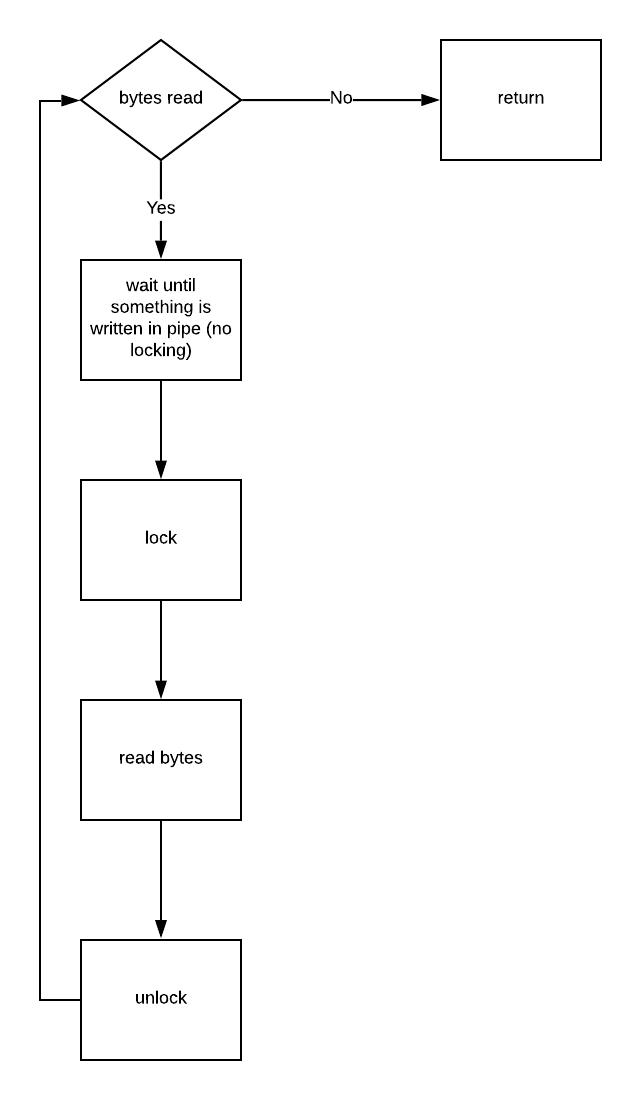
\includegraphics[scale=0.7]{figures/pipe_read.png}
\caption{pipe read flow chart\label{fig4_6}}
\end{figure}

Στην παραπάνω εικόνα ~\ref{fig4_6} φαίνεται το διάγραμμα ροής, όταν εκτελείται η
κλήση read σε άκρο ανάγνωσης του pipe. Ουσιαστικά πρόκειται για ένα while loop,
το οποίο τερματίζει υπό τέσσερις ορισμένες συνθήκες:
\begin{enumerate}
	\item Αν έχουν διαβαστεί όσα bytes ζήτησε η εφαρμογή
	\item Αν έχουν διαβαστεί όλα τα bytes από το pipe (ανεξάρτητα από τα
		πόσα ζήτησε η εφαρμογή) 
	\item Αν δεν υπάρχουν δεδομένα να διαβαστούν και όλα τα άκρα εγγραφής
		έχουν κλείσει
	\item Αν κάτι πάει στραβά κατά τη διαδικασία μεταφοράς δεδομένων από την
		κοινή μνήμη στην εφαρμογή.
\end{enumerate}
Για την αποφυγή deadlocks, αρχικά γίνεται έλεγχος για τη διαθεσιμότητα δεδομένων
στο pipe χωρίς την απόκτηση του γενικού κλειδώματος. Σε περίπτωση, που υπάρχουν
δεδομένα, τότε αποκτάται το κλείδωμα και επαναλαμβάνεται ο έλεγχος με την κατοχή
του κλειδώματος. Αφού λοιπόν μεταφερθύν τα δεδομένα από την κοινή μνήμη στην
εφαρμογή, τότε ενημερώνονται οι κοινές μεταβλητές του pipe (out, cnt) και
ελευθερώνεται το lock. Καθώς ο buffer του pipe είναι κυκλικός, πρέπει να
λαμβάνουμε υπόψιν την περίπτωση που έχουμε φτάσει στο τέλος του buffer, οπότε
πρέπει να ξεκινήσουμε να διαβάζουμε τα υπόλοιπα δεδομένα από την αρχή. Τέλος,
τόσο κατά τη διάρκεια του ελέγχου δεδομένων χωρίς αλλά και με το κλείδωμα,
ελέγχονται και τα ανοιχτά άκρα εγγραφής στο pipe. Αν όλα έχουν κλείσει τότε
πρέπει να επιστρέψει η κλήση pipe καθώς δεν πρόκειται να εγγραφούν νέα δεδομένα.

\begin{figure}[htp]
\centering
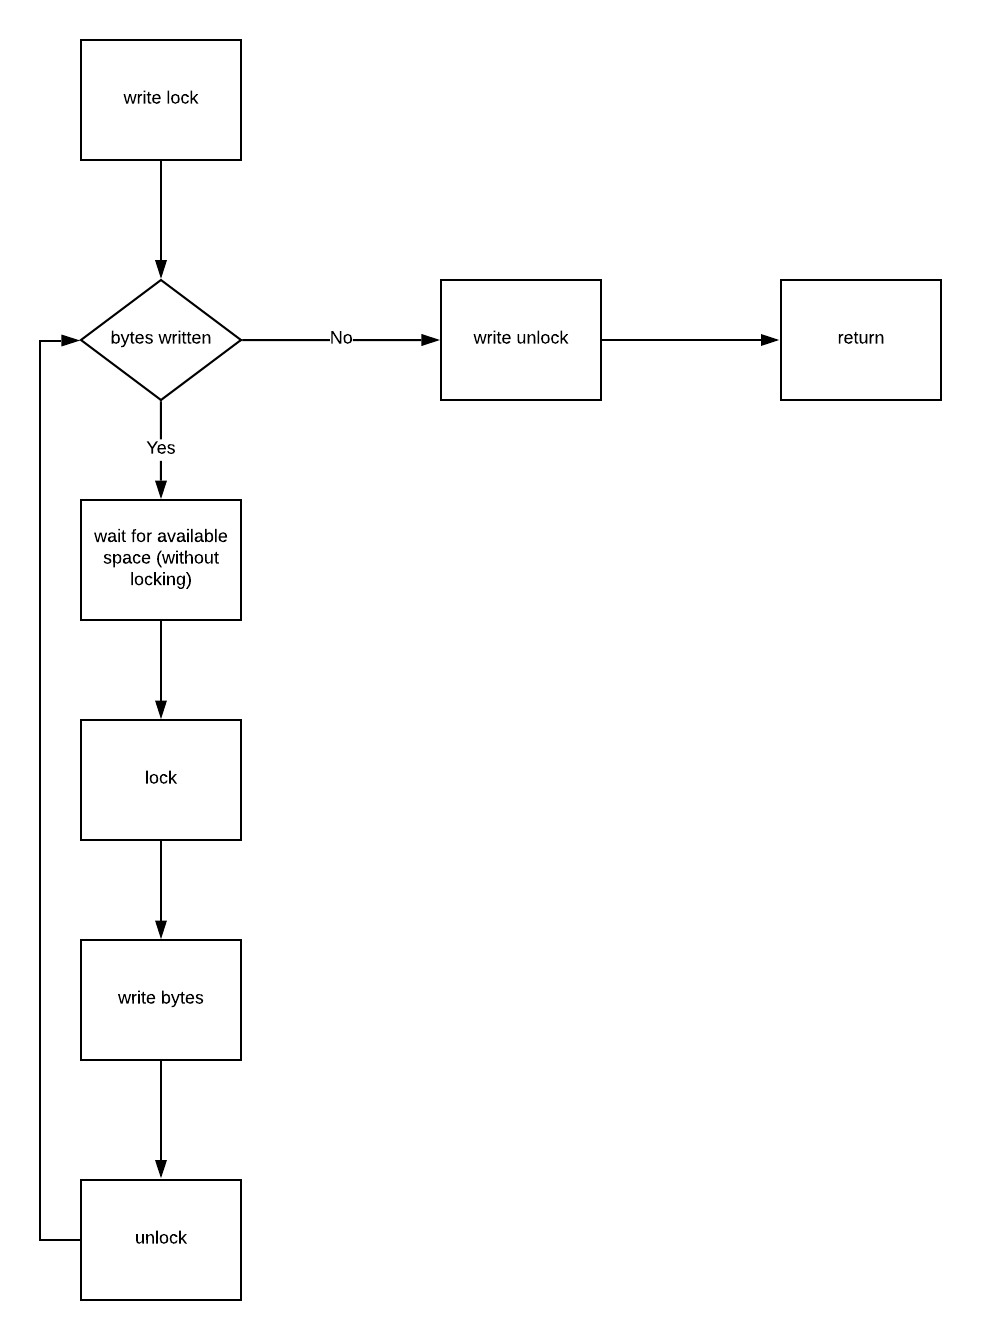
\includegraphics[scale=0.7]{figures/pipe_write.png}
\caption{pipe write flow chart\label{fig4_7}}
\end{figure}

Στην παραπάνω εικόνα ~\ref{fig4_7} φαίνεται το διάγραμμα ροής της κλήσης write
του pipe. Όπως φαίνεται δεν έχει κάποια ιδιαίτερη διαφορά με το διάγραμμα ροής
της κλήσης read, εκτός από το γεγονός ότι από την αρχή μέχρι το τέλος της
εκτέλεσης της δεσμεύεται το wr\_lock. Ο λόγος ύπαρξης ενός τέτοιου κλειδώματος,
είναι για να επιτευχθεί η ατομικότητα της κλήσης write σε ένα pipe. Από εκεί και
πέρα, όπως και πριν αρχικά ελέγχουμε αν υπάρχει διαθέσιμος χώρος στην κοινή
μνήμη για την εισαγωγή νέων δεδομένων. Έπειτα αποκτάται το κλείδωμα και
επαναλαμβάνεται ο έλεγχος διαθέσιμου χώρου. Αν είναι επιτυχής, γίνεται η εγγραφή
δεδομένων στην κοινή μνήμη και ενημερώνονται οι αντίστοιχες μεταβλητές (in,
cnt). Καθώς οbuffer του pipe είναι κυκλικός πρέπει να λαμβάνουμε υπόψιν την
περίπτωση που ο διαθέσιμος χώρος βρίσκεται την αρχή του buffer. Τόσο κατά τη
διαδικασία ελέγχου διαθέσιμου χώρου χωρίσς κλείδωμα όσο και με κλείδωμα,
ελέγχονται και τα ανοιχτά άκρας ανάγνωσης του pipe. Αν όλα έχουν κλείσει τότε
πρέπει να επιστρέψει η κλήση pipe με το error EPIPE, καθώς δεν υπάρχουν
αναγνώστες να διαβάσουν τα δεδομένα. Τέλος, ´ολα τα παραπάνω βρίσκονται μέσα σε
ένα while loop το οποίο μπορεί να τερματίσει υπό τις τέσσερις παρακάτω συνθήκες.
\begin{enumerate}
	\item Αν έχουν γραφτεί όσα bytes ζήτησε η εφαρμογή
	\item Αν δεν υπάρχει κανένα ανοιχτό άκρο ανάγνωσης στο pipe.
	\item Αν κάτι πάει στραβά κατά τη διαδικασία μεταφοράς δεδομένων από την
		την εφαρμογή στην κοινή μνήμη.
\end{enumerate}

\subsection{Στάδια υλοποίησης}




\chapter{Επίλογος}
μπλα μπλα μπλα

\section{Mpla}
dsfdsgfdsgdfs

\section{Mpla}
dsfdsgfdsgdfs
\subsection{Mpla}
dsfdsgfdsgdfs





mpla ~\cite{gao2017containerleaks}

\bibliographystyle{plain}
\bibliography{ref}{}
\end{document}

